\documentclass[journal=jacsat,manuscript=article]{achemso}
%\documentclass{article}


\usepackage{graphicx}
\usepackage[version=3]{mhchem} % Formula subscripts using \ce{}
\usepackage{amsmath}
\usepackage{graphicx}
\usepackage{wrapfig}
\usepackage{longtable}
\usepackage{placeins}
\usepackage{color,soul}
\usepackage[colorinlistoftodos]{todonotes}
%\usepackage[colorlinks=true, allcolors=blue]{hyperref}
\usepackage{subcaption}
\usepackage{comment}
\usepackage{totcount}
\usepackage{makecell}
\usepackage{lastpage}
\usepackage{array}
\setlength\extrarowheight{2pt}
\renewcommand{\thefigure}{\arabic{figure}S}
\renewcommand{\thefigure}{S\arabic{figure}}

\title{Supplementary Information for Computational Study of Transition-Metal Substitutions in Rutile TiO$_2$ (110) for Photoelectrocatalytic Ammonia Synthesis}

\affiliation{$^{1}$ School of Chemical and Biomolecular Engineering, Georgia Institute of Technology\\
$^{2}$ School of Materials Science and Engineering, Georgia Institute of Technology\\
$^{3}$ School of Physics, Georgia Institute of Technology\\
$^{4}$ School of Computer Science, Georgia Institute of Technology\\
$\dagger$ These authors contributed equally to this work. \\
* Correspondence \email{andrew.medford@chbe.gatech.edu}\\
  311 Ferst Drive NW, Atlanta, Georgia 30318 \\
  Tel.:+1 (404) 385-5531\\}
\email{andrew.medford@chbe.gatech.edu}
\phone{+1 (404) 385-5531}

\author{Benjamin M. Comer$^{1 \dagger}$, Max H. Lenk$^{2 \dagger}$, Aradhya P. Rajanala$^{3}$, Emma L. Flynn$^{4}$, Andrew J. Medford$^{1}$*}
\begin{document}

\maketitle\begin{table}
\setlength\tabcolsep{2pt}
\begin{center}
\begin{tabular}{| c | c | c | c | c | c | c | c | c | c | c | c | c | c |}
\hline
Element & H$_2$NNH$_2$ & HNNH & N & N$_2$ & N$_2$H & N$_2$H$_2$ & N$_2$H$_3$ & NH & NH$_2$ & NH$_3$ & Formation Energy\\
\hline

Pd & 1.53 & 2.12 & 3.55 & 0.23 & 2.0 & 2.25 & 1.67 & 2.5 & 0.26 & -0.22 & 6.08 \\
V & 1.43 & 1.5 & -0.33 & 0.04 & 0.82 & 0.38 & 0.55 & 0.17 & -1.04 & -1.03 & 2.48 \\
Mo & 1.27 & 1.11 & -1.2 & -0.33 & 0.01 & -0.08 & 0.39 & -0.24 & -1.2 & -0.75 & 3.26 \\
Hf & 1.21 & 1.32 & 1.59 & -0.02 & 0.97 & 0.6 & 0.2 & 0.02 & -1.44 & -0.95 & -0.92 \\
Pt &  & 2.16 & 2.77 & 0.26 & 1.78 & 2.06 & 1.44 & 1.69 & -0.1 & -0.09 & 6.86 \\
Zr & 1.23 & 1.39 & 1.71 & -0.01 & 1.07 & 0.74 & 0.35 & 0.16 & -1.26 & -0.88 & -0.51 \\
Sc & 1.06 & 1.76 & 3.51 & 0.03 & 1.7 & 1.59 & 1.0 & 2.18 & -0.6 & -0.76 & -1.71 \\
W & 1.25 & 0.84 & -1.8 & -0.37 & -0.24 & -0.73 & 0.01 & -1.06 & -1.6 & -0.8 & 3.99 \\
Ru & 0.82 & 0.76 & 0.48 & -0.83 & 0.64 & 0.17 & 0.57 & 0.86 & -0.93 & -1.13 & 5.45 \\
Ta & 1.1 & 0.31 & -0.99 & -0.13 & 0.42 & -0.32 & -0.22 & -0.95 & -1.86 & -0.85 & 1.69 \\
Ti & 1.42 & 1.64 & 1.73 & 0.11 & 1.27 & 0.85 & 0.61 & 0.37 & -0.99 & -0.6 & 0.0 \\
Co & 1.14 & 1.53 & 2.34 & 0.12 & 1.04 & 1.05 & 0.78 & 1.82 & -0.74 & -0.72 & 4.49 \\
Nb & 1.23 & 0.43 & -1.04 & -0.23 & 0.35 & -0.36 & -0.04 & -0.84 & -1.7 & -0.86 & 1.5 \\
Ir & 0.82 & 0.74 & 1.03 & -0.7 & 0.26 & 0.19 & -0.01 & 0.54 & -1.52 & -1.2 & 7.07 \\
Rh & 1.16 & 1.3 & 1.86 & -0.16 & 0.71 & 0.85 & 0.44 & 1.34 & -1.06 & -0.87 & 6.01 \\
Y & 1.01 & 1.69 & 2.72 & 0.02 &  & 2.0 & 1.34 & 2.58 & -0.15 & -0.77 & -1.38 \\
Cu & 1.33 & 2.07 & 4.51 & 0.18 & 2.33 & 2.4 & 1.65 & 3.41 & 0.78 & -0.45 & 6.55 \\
Ag & 1.44 & 2.33 & 5.3 & 0.24 & 2.62 & 2.65 & 2.04 & 3.83 & 1.11 & -0.18 & 7.28 \\
Ni & 1.75 & 1.94 & 3.35 & 0.17 & 1.64 & 1.9 & 1.09 &  & -0.06 & -0.43 & 5.58 \\
Tc & 1.03 & 0.95 & -0.87 & -0.65 & 0.06 & 0.27 & 0.65 & 0.52 & -0.87 & -0.92 & 4.58 \\
Os & 0.61 & 0.39 & -0.7 & -1.17 & -0.15 & -0.36 & 0.06 & 0.06 & -1.44 & -1.29 & 6.31 \\
Au & 1.68 & 2.36 & 4.05 & 0.25 & 2.54 & 2.82 & 2.15 & 2.95 & 0.75 & -0.08 & 8.18 \\
Re & 0.95 & 0.67 & -1.5 & -0.83 & -0.42 & -0.15 & 0.32 & -0.18 & -1.21 & -0.96 & 5.06 \\
\hline
\end{tabular}
\end{center}
\caption{The calculated relative energies of all 2+ surface species on all metal substituents at standard state. All energies are referenced with respect to N$_2$ gas and H$_2$ gas at 300K and 1 bar of pressure. Blank spaces represent calculations that could not be converged}
\label{table:energies}
\end{table}

\begin{table}
\begin{center}
\begin{tabular}{| c | c | c | c |}
\hline
Element & N$_2$ & N$_2$H & Formation Energy \\
\hline
Pd & -0.01 & 1.7 & 9.88 \\
V & 0.19 & 2.81 & 2.82 \\
Mo & 0.14 &  & 3.95 \\
Fe & -0.12 &  & 8.4 \\
Hf & 0.06 & 2.43 & -1.22 \\
Pt & -0.34 & 1.77 & 10.08 \\
Zr & 0.07 & 2.46 & -0.75 \\
Sc & 0.08 & 2.34 & 0.63 \\
W & 0.13 & 2.37 & 4.36 \\
Ru & -0.0 &  & 7.5 \\
Ta & 0.1 & 2.37 & 1.39 \\
Ti & 0.16 & 2.54 & -0.0 \\
Co & 0.2 &  & 7.42 \\
Nb & 0.11 & 2.45 & 1.4 \\
Ir & -0.39 & 2.1 & 9.12 \\
Rh & -0.14 & 2.22 & 8.71 \\
Y & 0.04 & 2.6 & 1.1 \\
Cu & 0.22 &  & 10.16 \\
Ag & 0.24 &  & 11.09 \\
Ni & 0.2 & 1.75 & 9.29 \\
Tc & 0.12 &  & 5.88 \\
Os & -0.22 & 1.96 & 7.69 \\
Au & 0.27 & 2.23 & 11.22 \\
Re & 0.12 &  & 5.9 \\
\hline
\end{tabular}
\end{center}
\label{table:4+_energies}
\caption{The calculated relative energies of all 4+ surface species on all metal substituents at standard state. All energies are referenced with respect to N$_2$ gas and H$_2$ gas at 300K and 1 bar of pressure. Blank spaces represent calculations that could not be converged}
\end{table}

\begin{table}
\begin{center}
\begin{tabular}{| c | c |c |}
\hline
Element & Limiting Potential & Limiting Step \\
\hline
Sc & -1.7 & N$_2$ $\rightarrow$ N$_2$H*\\
Ti & -1.27 & N$_2$ $\rightarrow$ N$_2$H*\\
V & -0.82 & N$_2$ $\rightarrow$ N$_2$H*\\
Co & -1.04 & N$_2$ $\rightarrow$ N$_2$H*\\
Ni & -1.64 & N$_2$ $\rightarrow$ N$_2$H*\\
Cu & -2.33 & N$_2$ $\rightarrow$ N$_2$H*\\
Zr & -1.08 & N$_2$* $\rightarrow$ N$_2$H*\\
Nb & -1.38 & NH$_2$*+NH$_3$ $\rightarrow$ 2NH$_3$\\
Mo & -0.89 & NH$_2$*+NH$_3$ $\rightarrow$ 2NH$_3$\\
Tc & -0.71 & N$_2$* $\rightarrow$ N$_2$H*\\
Ru & -1.47 & N$_2$* $\rightarrow$ N$_2$H*\\
Rh & -0.88 & N$_2$* $\rightarrow$ N$_2$H*\\
Pd & -2.0 & N$_2$ $\rightarrow$ N$_2$H*\\
Ag & -2.62 & N$_2$ $\rightarrow$ N$_2$H*\\
Hf & -1.12 & NH$_2$*+NH$_3$ $\rightarrow$ 2NH$_3$\\
Ta & -1.55 & NH$_2$*+NH$_3$ $\rightarrow$ 2NH$_3$\\
W & -1.29 & NH$_2$*+NH$_3$ $\rightarrow$ 2NH$_3$\\
Re & -0.9 & NH$_2$*+NH$_3$ $\rightarrow$ 2NH$_3$\\
Os & -1.12 & NH$_2$*+NH$_3$ $\rightarrow$ 2NH$_3$\\
Ir & -1.2 & NH$_2$*+NH$_3$ $\rightarrow$ 2NH$_3$\\
Au & -2.54 & N$_2$ $\rightarrow$ N$_2$H*\\
\hline
\end{tabular}
\end{center}
\caption{The limiting potentials and limiting steps for each dopant metal on 2+ surfaces}\label{table:pot_limiting_steps}\end{table}\begin{table}
\begin{center}
\begin{tabular}{| c | c |c |}
\hline
Element & Largest Thermodynamic Step & Limiting Step \\
\hline
Sc & 0.44 & NH$_3$*+NH$_3$ $\rightarrow$ 2NH$_3$\\
Ti & 0.68 & NH$_3$*+NH$_3$ $\rightarrow$ 2NH$_3$\\
V & 0.72 & NH$_3$*+NH$_3$ $\rightarrow$ 2NH$_3$\\
Co & 0.43 & NH$_3$*+NH$_3$ $\rightarrow$ 2NH$_3$\\
Ni & 0.17 & N$_2$ $\rightarrow$ N$_2$*\\
Cu & 1.25 & H$_2$NNH$_2$* $\rightarrow$ 2NH$_2$*\\
Zr & 0.95 & NH$_3$*+NH$_3$ $\rightarrow$ 2NH$_3$\\
Nb & 1.38 & NH$_3$*+NH$_3$ $\rightarrow$ 2NH$_3$\\
Mo & 0.89 & NH$_3$*+NH$_3$ $\rightarrow$ 2NH$_3$\\
Tc & 0.61 & NH$_3$*+NH$_3$ $\rightarrow$ 2NH$_3$\\
Ru & 0.82 & NH$_3$*+NH$_3$ $\rightarrow$ 2NH$_3$\\
Rh & 0.75 & NH$_3$*+NH$_3$ $\rightarrow$ 2NH$_3$\\
Pd & 0.54 & H$_2$NNH$_2$* $\rightarrow$ 2NH$_2$*\\
Ag & 1.48 & H$_2$NNH$_2$* $\rightarrow$ 2NH$_2$*\\
Hf & 1.12 & NH$_3$*+NH$_3$ $\rightarrow$ 2NH$_3$\\
Ta & 1.55 & NH$_3$*+NH$_3$ $\rightarrow$ 2NH$_3$\\
W & 1.29 & NH$_3$*+NH$_3$ $\rightarrow$ 2NH$_3$\\
Re & 0.9 & NH$_3$*+NH$_3$ $\rightarrow$ 2NH$_3$\\
Os & 1.12 & NH$_3$*+NH$_3$ $\rightarrow$ 2NH$_3$\\
Ir & 1.2 & NH$_3$*+NH$_3$ $\rightarrow$ 2NH$_3$\\
Au & 0.88 & H$_2$NNH$_2$* $\rightarrow$ 2NH$_2$*\\
\hline
\end{tabular}
\end{center}
\caption{The largest barrier for thermochemical steps and corresponding steps for each dopant metal on 2+ surfaces}\label{table:thermo_limiting_steps}\end{table}\begin{table}
\begin{center}
\begin{tabular}{| c | c |c |}
\hline
Element & Rate Limiting Step & Limiting Step \\
\hline
Sc & 1.56 & N$_2$ $\rightarrow$ N$_2$H*\\
Ti & 1.13 & N$_2$ $\rightarrow$ N$_2$H*\\
V & 0.76 & N$_2$H$_2$* $\rightarrow$ H$_2$NNH$_2$*\\
Co & 0.9 & N$_2$ $\rightarrow$ N$_2$H*\\
Ni & 1.62 & N$_2$ $\rightarrow$ N$_2$H$_2$*\\
Cu & 2.19 & N$_2$ $\rightarrow$ N$_2$H*\\
Zr & 0.94 & N$_2$* $\rightarrow$ N$_2$H*\\
Nb & 1.31 & N$_2$H$_2$* $\rightarrow$ H$_2$NNH$_2$*\\
Mo & 1.07 & N$_2$H$_2$* $\rightarrow$ H$_2$NNH$_2$*\\
Tc & 1.11 & N$_2$* $\rightarrow$ H$_2$NNH$_2$*\\
Ru & 1.33 & N$_2$* $\rightarrow$ N$_2$H*\\
Rh & 0.73 & N$_2$* $\rightarrow$ N$_2$H*\\
Pd & 1.96 & N$_2$ $\rightarrow$ N$_2$H$_2$*\\
Ag & 2.47 & N$_2$ $\rightarrow$ N$_2$H*\\
Hf & 0.98 & NH$_2$*+NH$_3$ $\rightarrow$ 2NH$_3$\\
Ta & 1.41 & NH$_2$*+NH$_3$ $\rightarrow$ 2NH$_3$\\
W & 1.69 & N$_2$H$_2$* $\rightarrow$ H$_2$NNH$_2$*\\
Re & 1.21 & N$_2$* $\rightarrow$ H$_2$NNH$_2$*\\
Os & 0.98 & NH$_2$*+NH$_3$ $\rightarrow$ 2NH$_3$\\
Ir & 1.06 & NH$_2$*+NH$_3$ $\rightarrow$ 2NH$_3$\\
Au & 2.54 & N$_2$ $\rightarrow$ N$_2$H$_2$*\\
\hline
\end{tabular}
\end{center}
\caption{The largest thermodynamic barrier and corresponding steps for each dopant metal on 2+ surfaces when set at the band edge of rutile, -0.142V}\label{table:rate_limiting_steps}\end{table}\begin{figure}
\centering
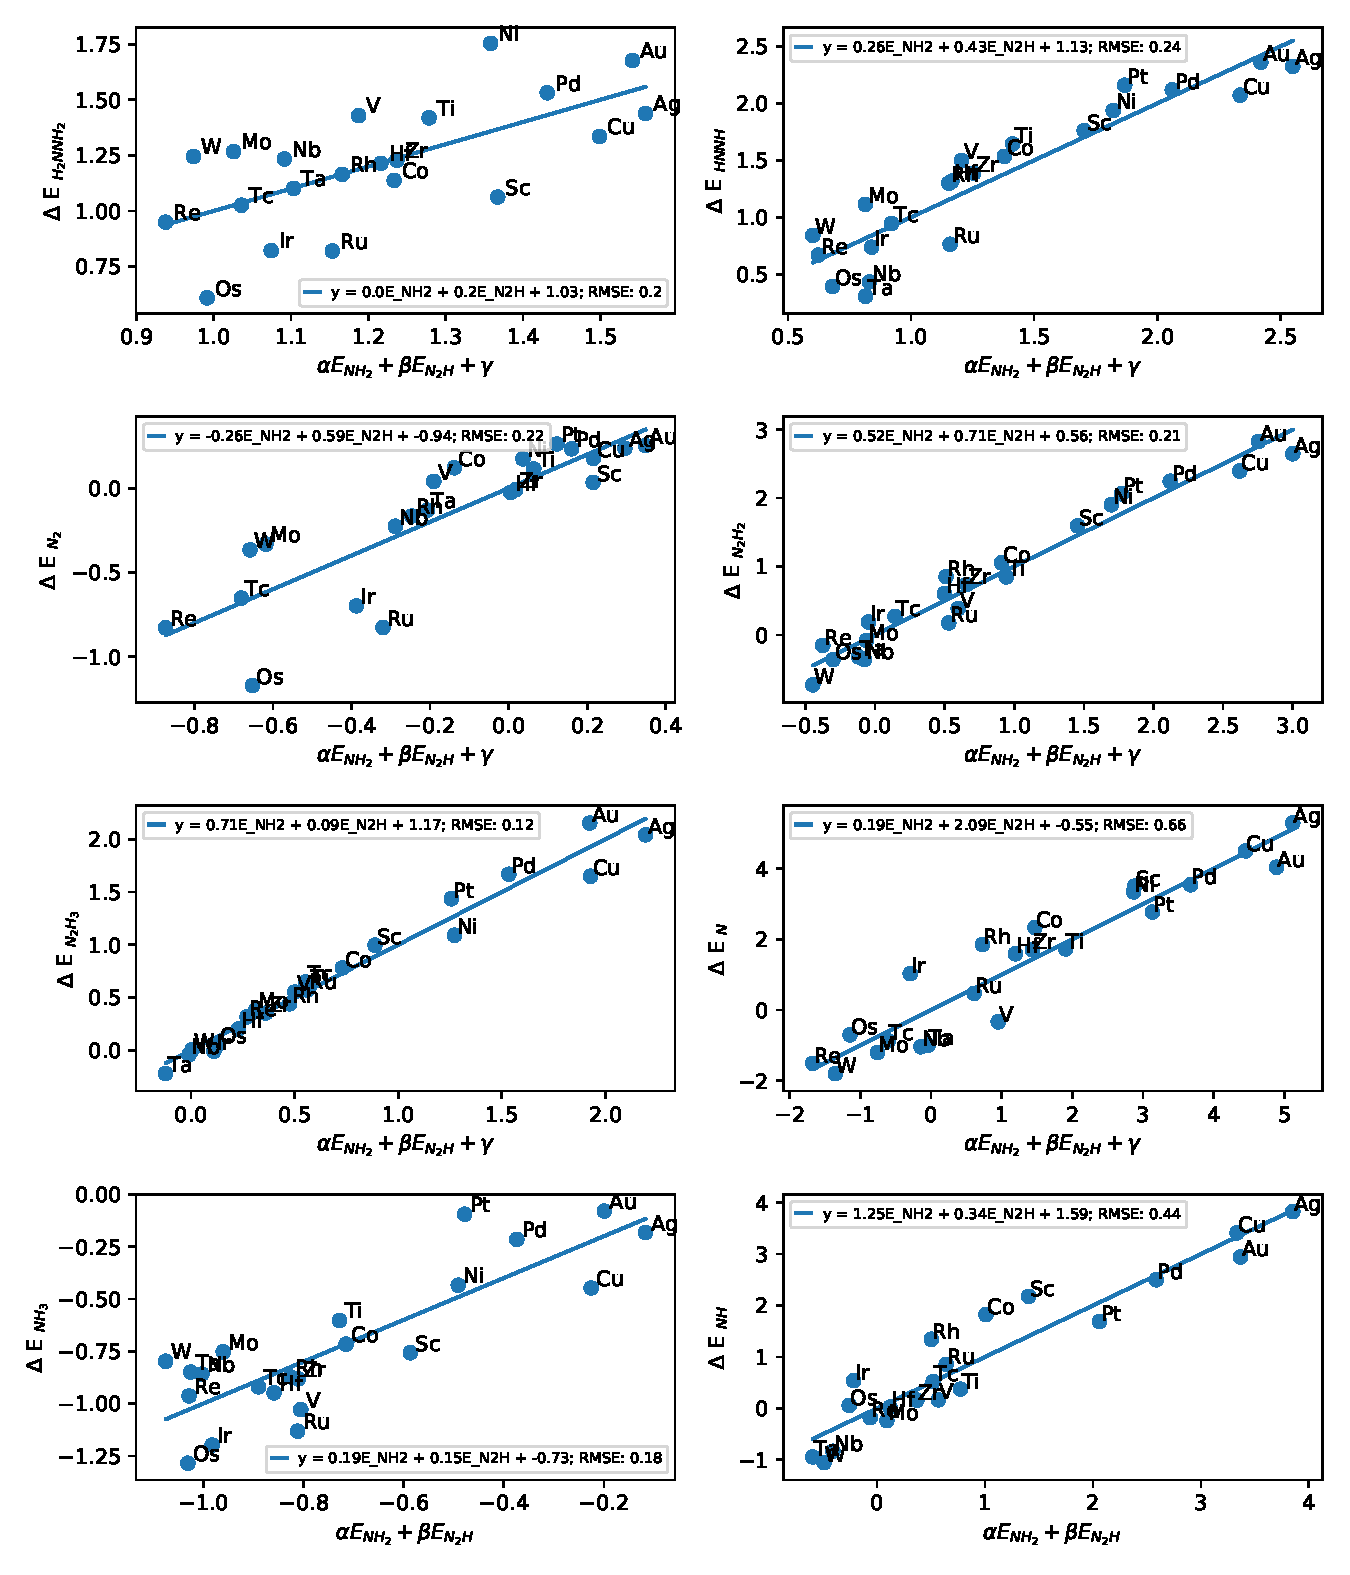
\includegraphics[width=0.8\linewidth]{Images/scaling_species.pdf}
\caption{The calculated scaling relations between the binding energies of various species and the binding energies of N$_2$H and NH$_2$ on 2+ dopant sites}
\label{fig:scaling_species}
\end{figure}

\begin{figure}
\centering
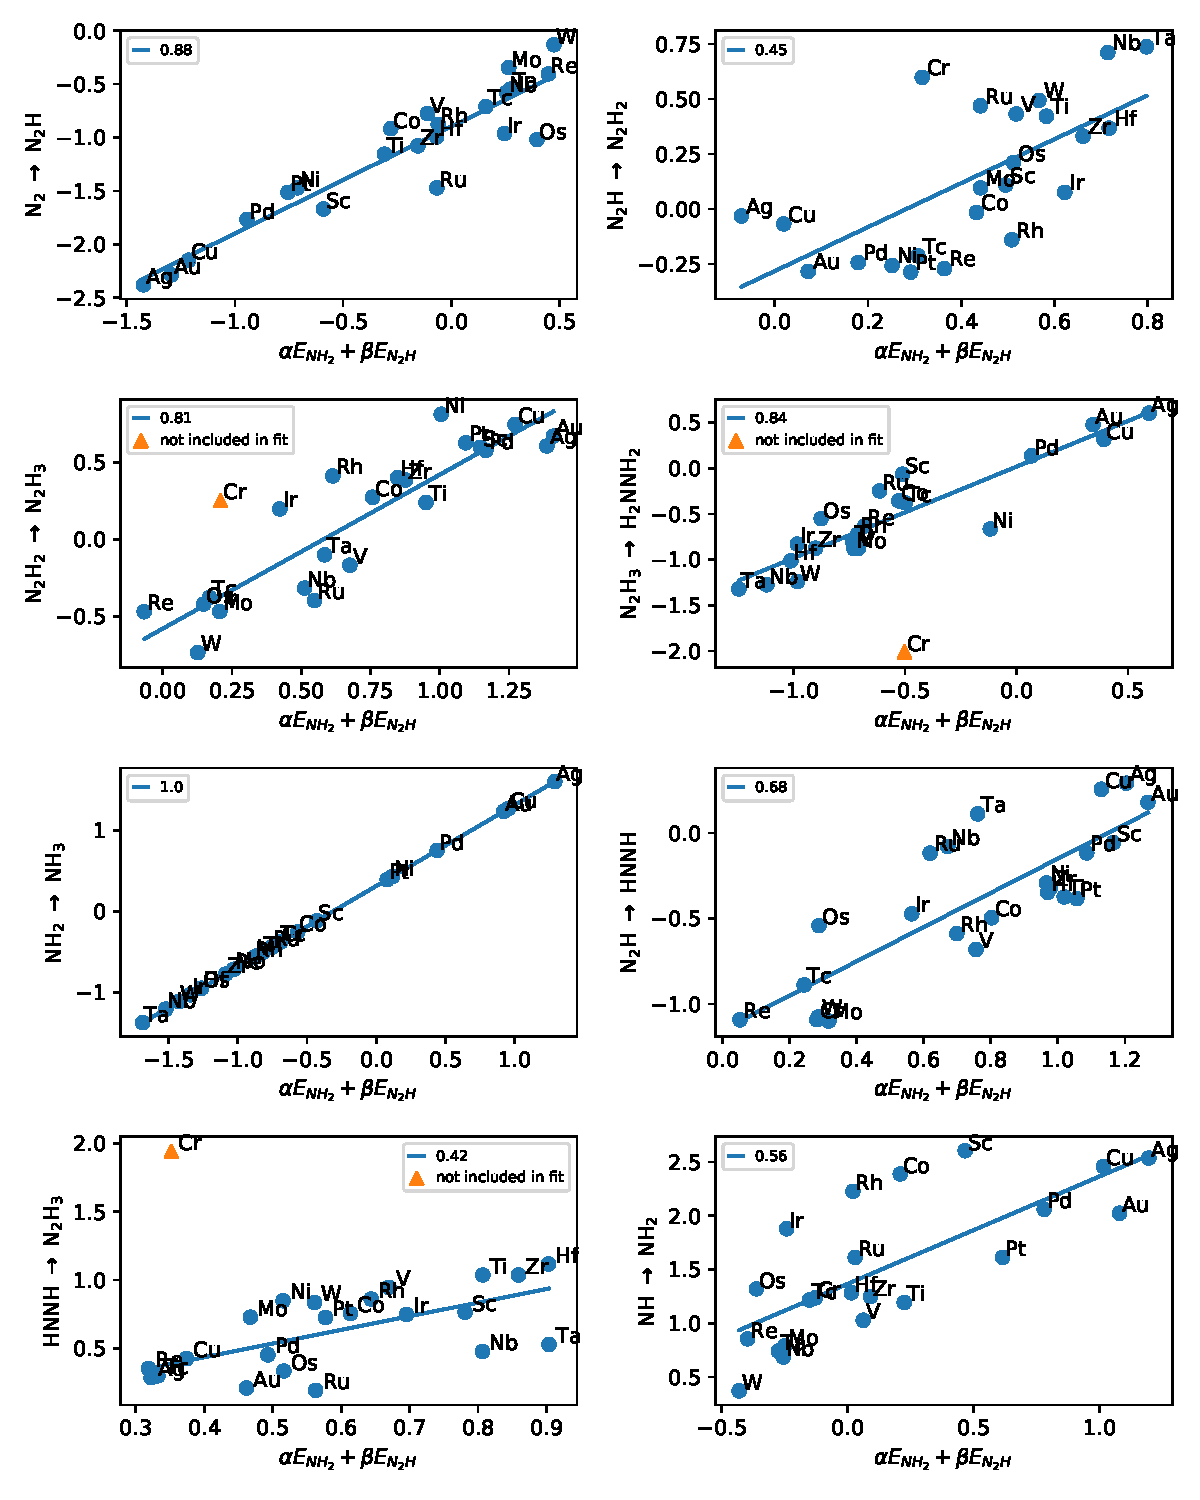
\includegraphics[width=0.8\linewidth]{Images/scaling_reactions.pdf}
\caption{The calculated scaling relations between the reaction energies energies of all electrochemical reations and the binding energies of N$_2$H and NH$_2$ on 2+ dopant sites}
\label{fig:scaling_reactions}
\end{figure}

\begin{figure}
\centering
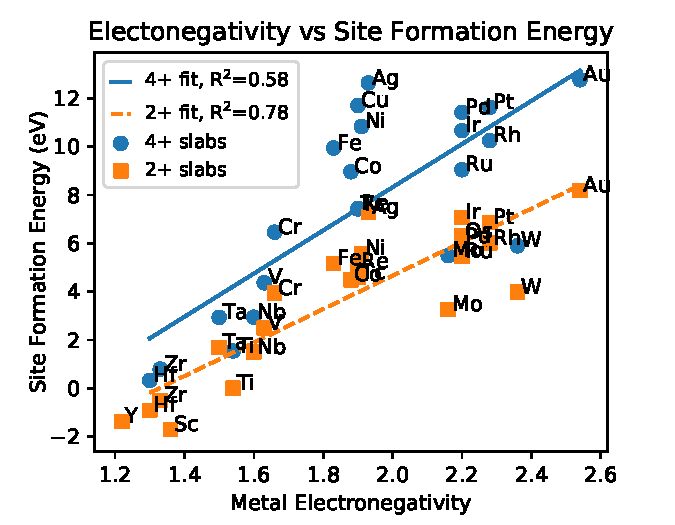
\includegraphics[width=0.8\linewidth]{Images/electronegativity_vs_formation.pdf}
\caption{Electronegativity vs formation energy of 2+ dopant site}
\label{fig:electronegativity}
\end{figure}

\begin{figure}
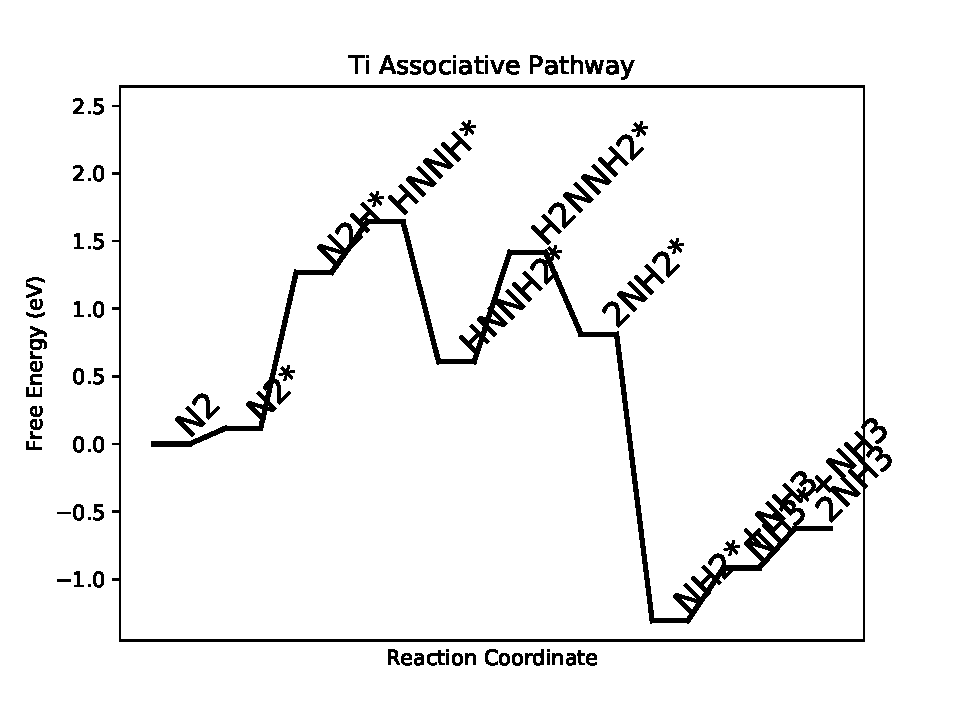
\includegraphics[width=0.5\linewidth]{data/plots/Ti_associative.pdf}
\label{fig:Ti_associative}
\end{figure}

\begin{figure}
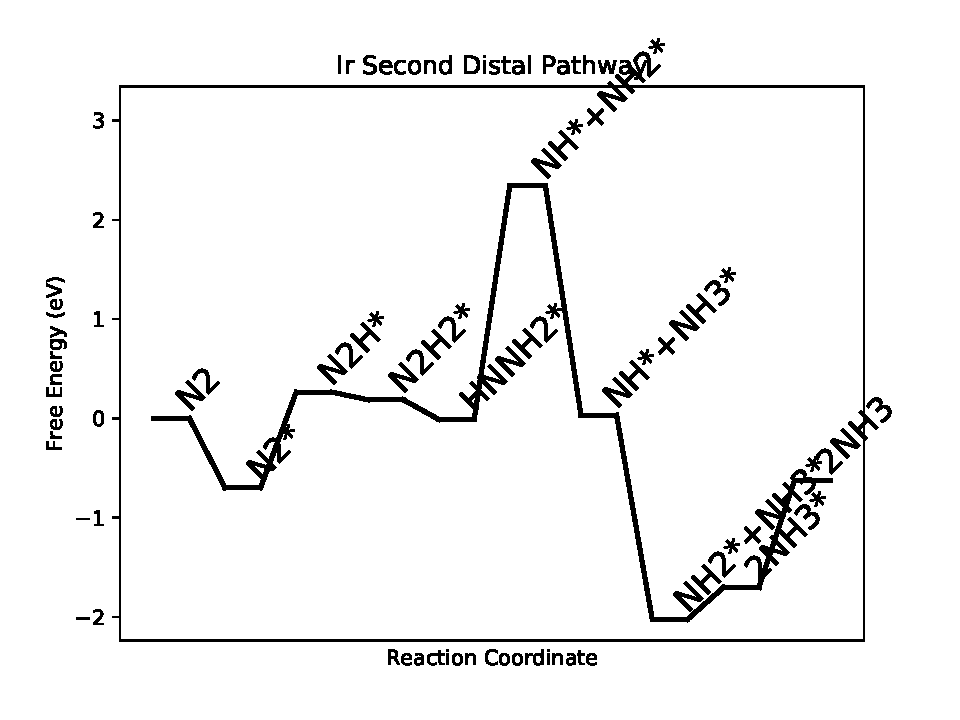
\includegraphics[width=0.5\linewidth]{data/plots/Ir_distal_2.pdf}
\label{fig:Ir_distal_2}
\end{figure}

\begin{figure}
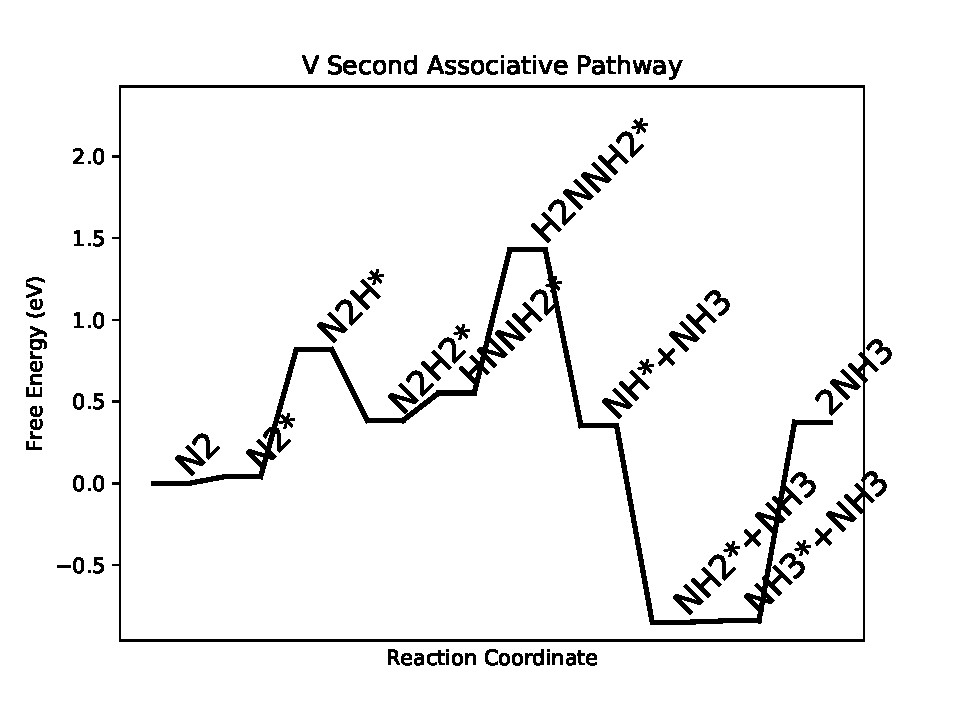
\includegraphics[width=0.5\linewidth]{data/plots/V_associative_2.pdf}
\label{fig:V_associative_2}
\end{figure}

\begin{figure}
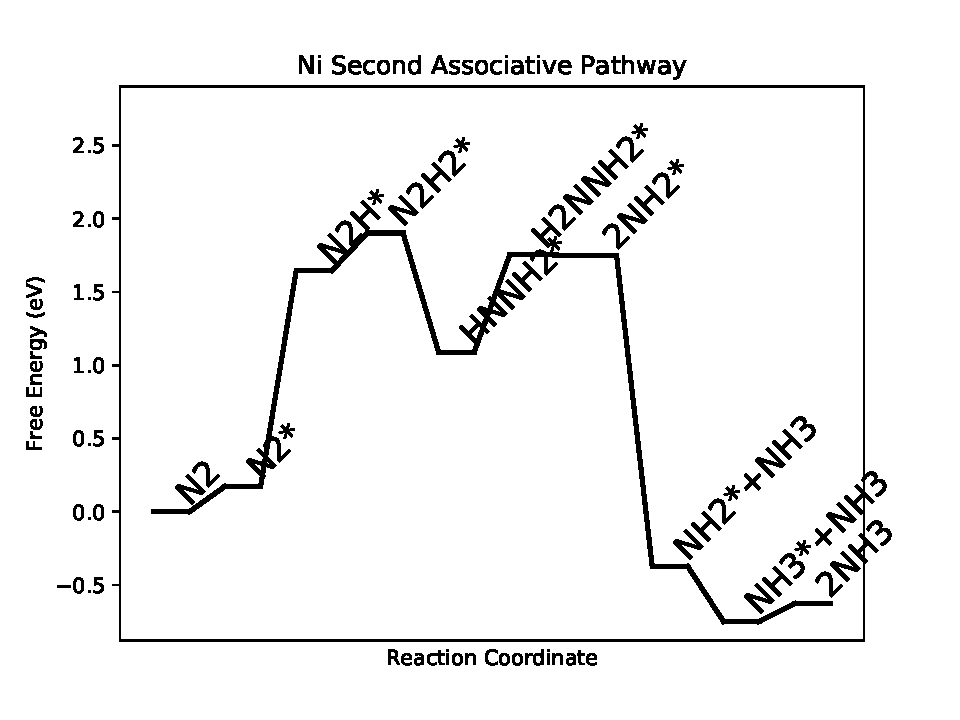
\includegraphics[width=0.5\linewidth]{data/plots/Ni_associative_2.pdf}
\label{fig:Ni_associative_2}
\end{figure}

\begin{figure}
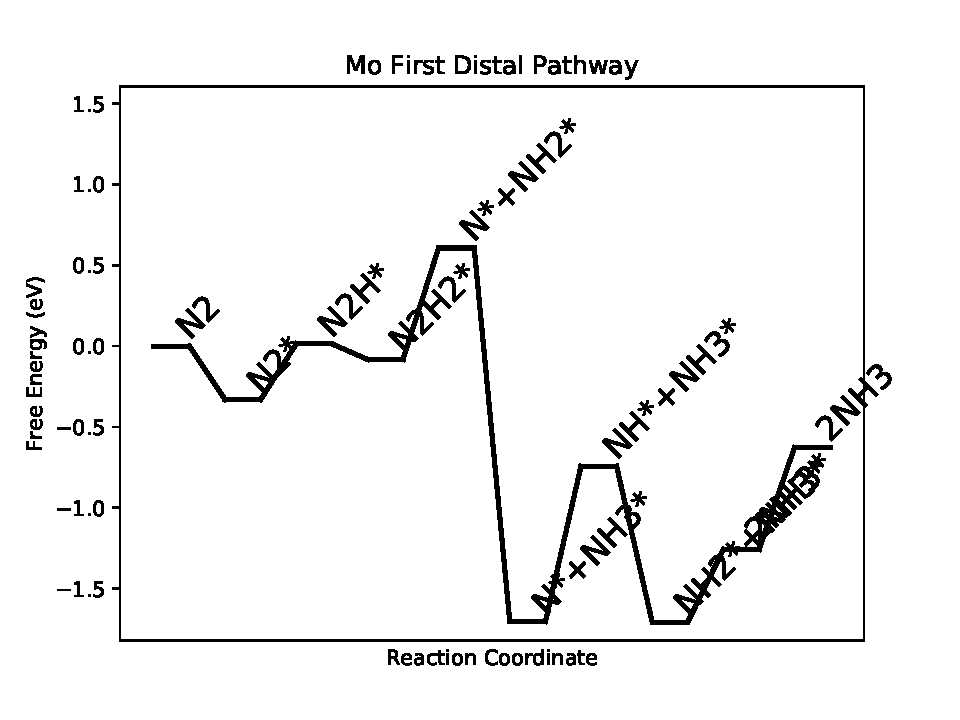
\includegraphics[width=0.5\linewidth]{data/plots/Mo_distal_1.pdf}
\label{fig:Mo_distal_1}
\end{figure}

\begin{figure}
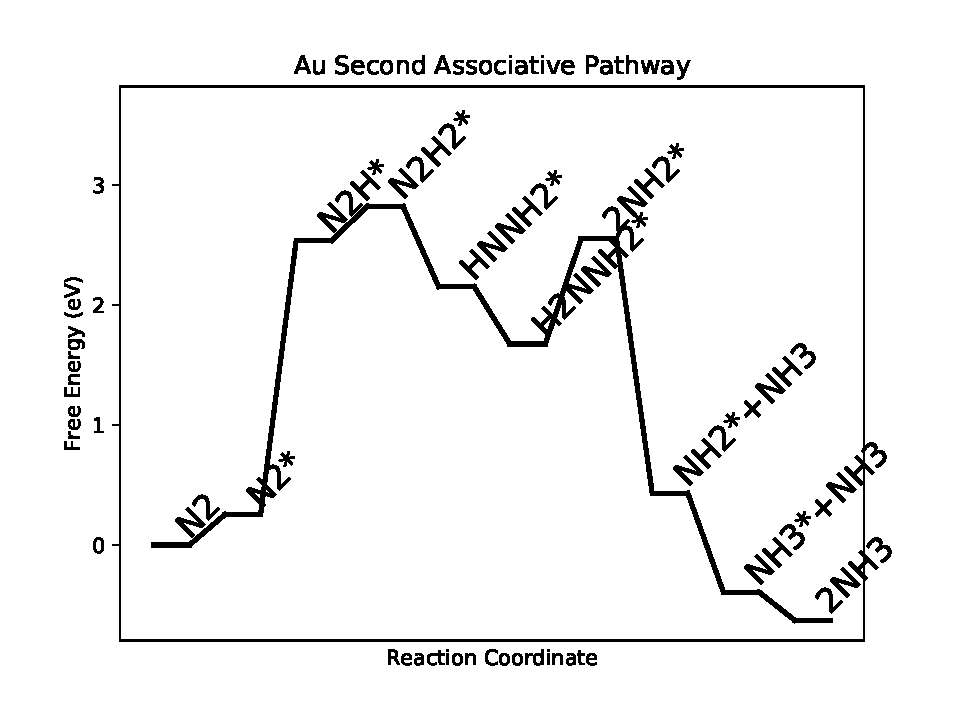
\includegraphics[width=0.5\linewidth]{data/plots/Au_associative_2.pdf}
\label{fig:Au_associative_2}
\end{figure}

\begin{figure}
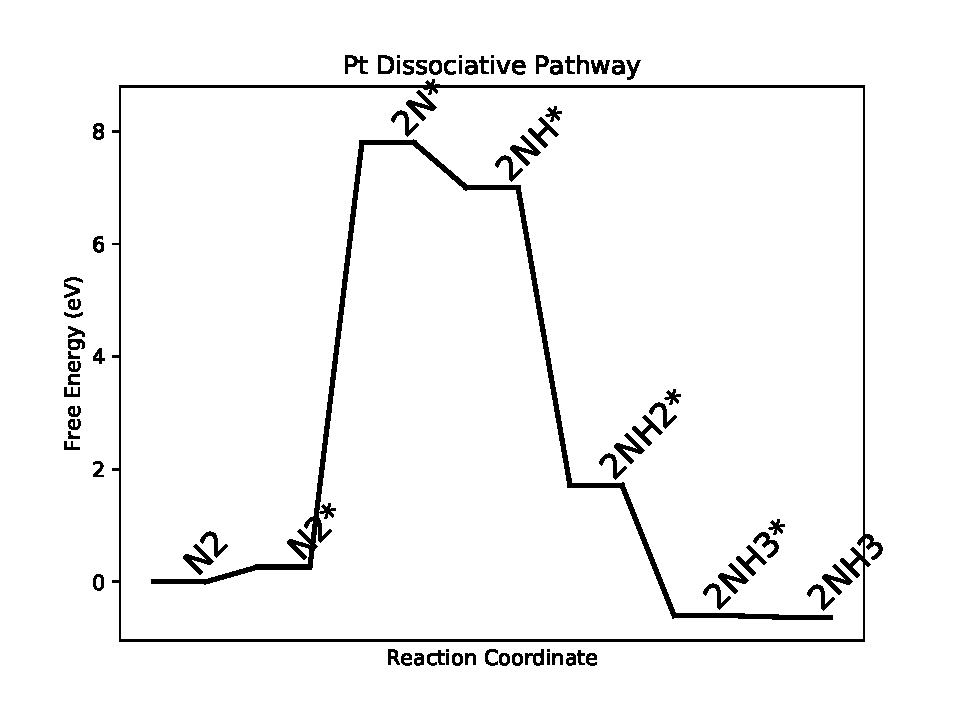
\includegraphics[width=0.5\linewidth]{data/plots/Pt_dissociative.pdf}
\label{fig:Pt_dissociative}
\end{figure}

\begin{figure}
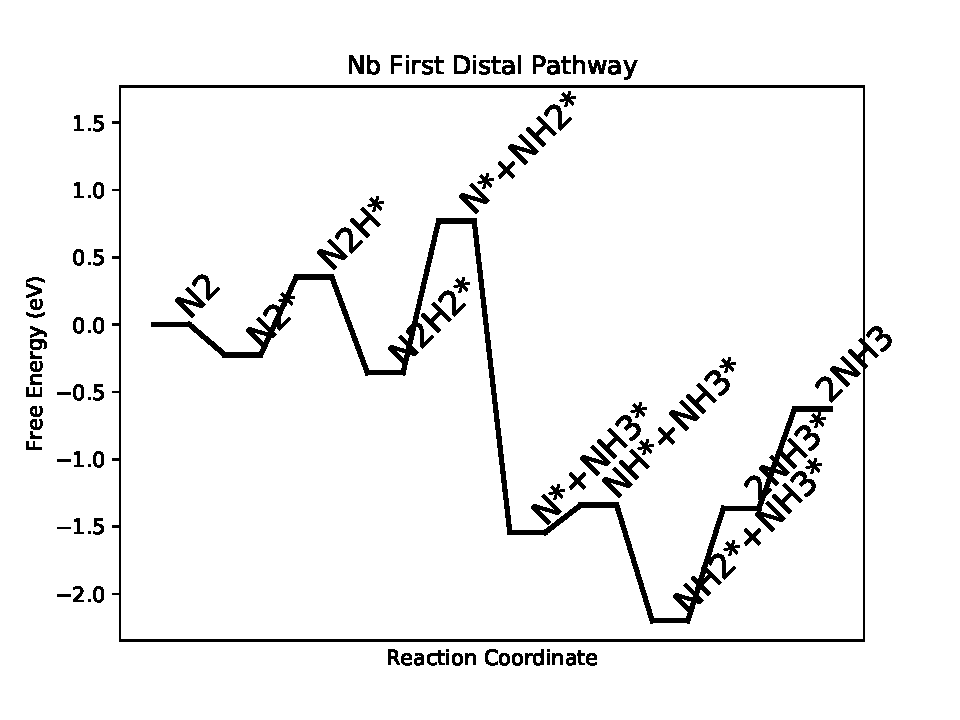
\includegraphics[width=0.5\linewidth]{data/plots/Nb_distal_1.pdf}
\label{fig:Nb_distal_1}
\end{figure}

\begin{figure}
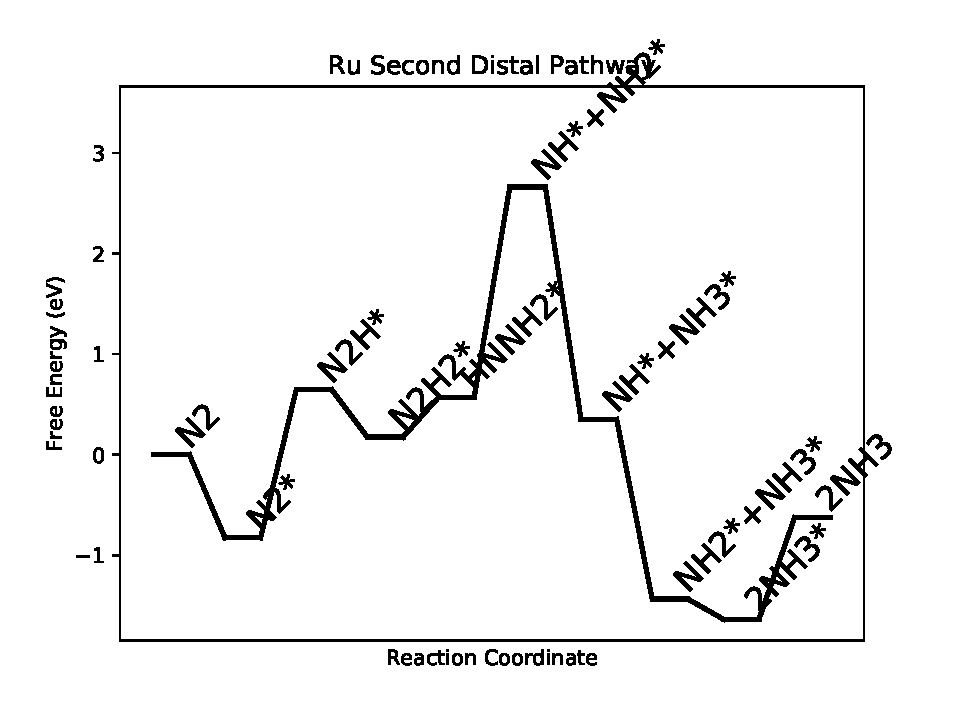
\includegraphics[width=0.5\linewidth]{data/plots/Ru_distal_2.pdf}
\label{fig:Ru_distal_2}
\end{figure}

\begin{figure}
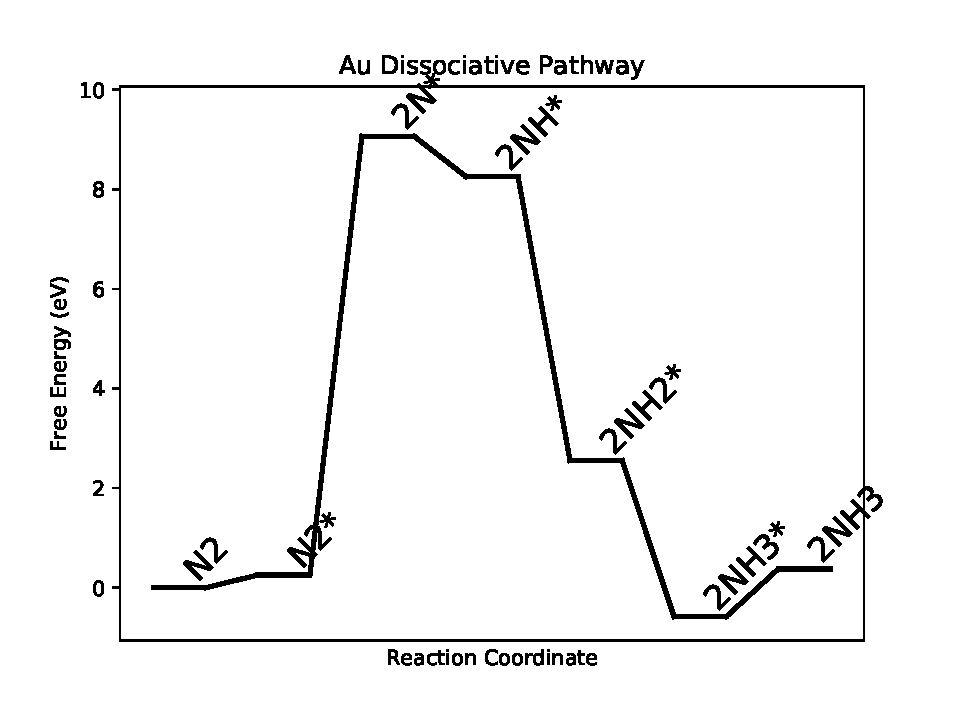
\includegraphics[width=0.5\linewidth]{data/plots/Au_dissociative.pdf}
\label{fig:Au_dissociative}
\end{figure}

\begin{figure}
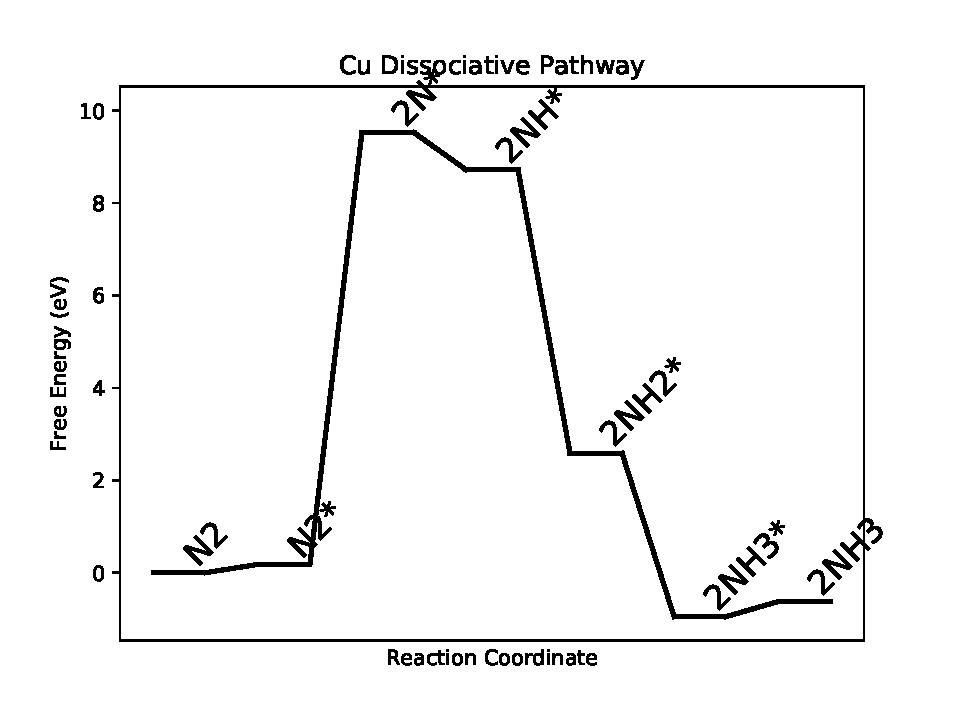
\includegraphics[width=0.5\linewidth]{data/plots/Cu_dissociative.pdf}
\label{fig:Cu_dissociative}
\end{figure}

\begin{figure}
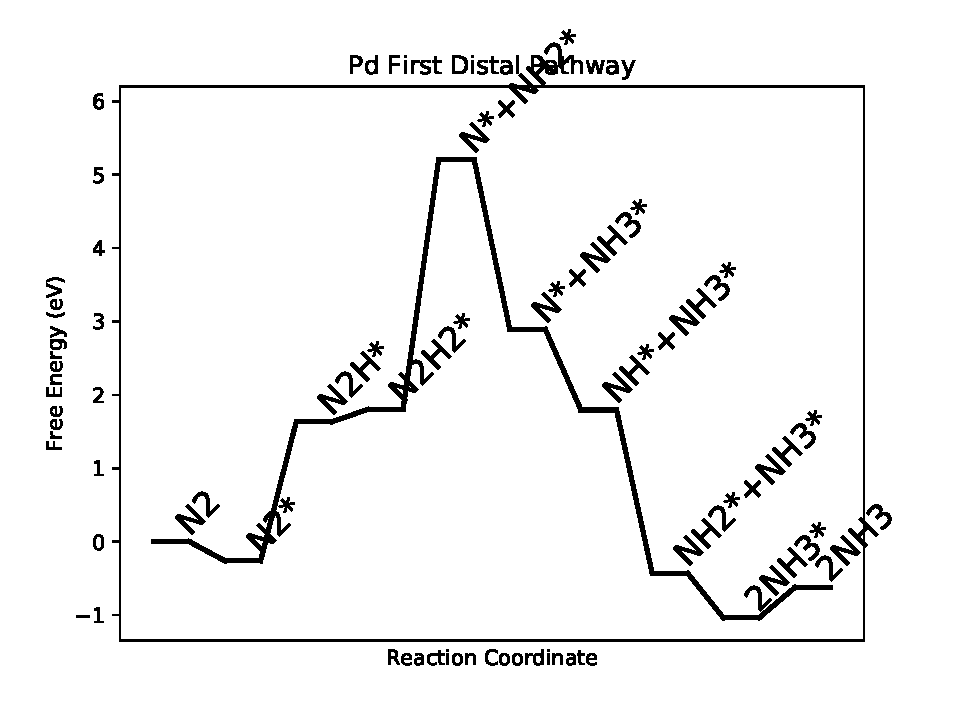
\includegraphics[width=0.5\linewidth]{data/plots/Pd_distal_1.pdf}
\label{fig:Pd_distal_1}
\end{figure}

\begin{figure}
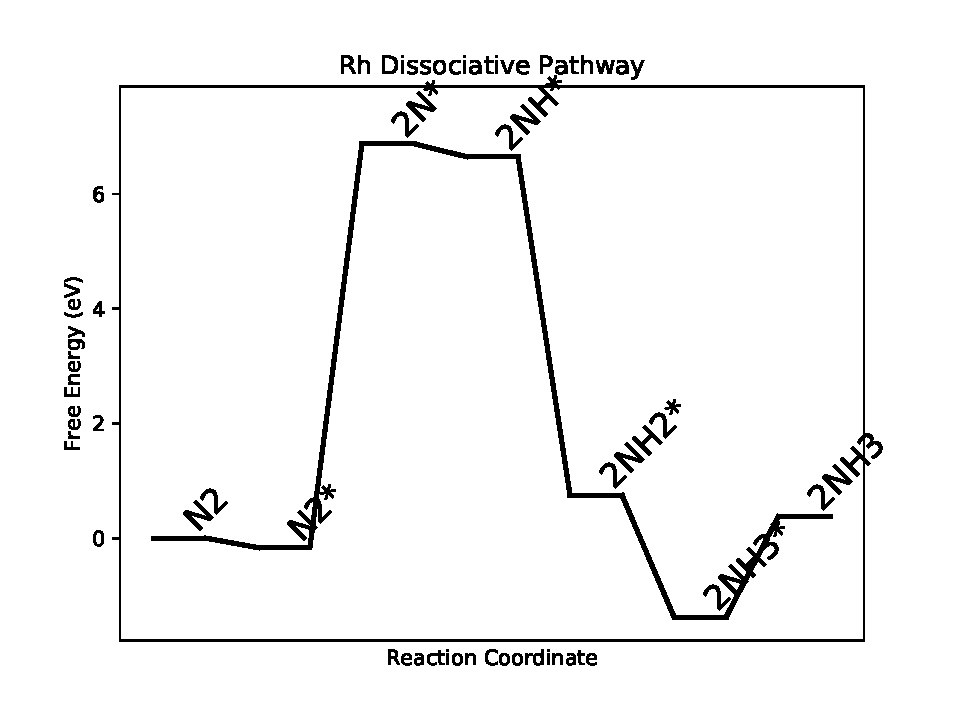
\includegraphics[width=0.5\linewidth]{data/plots/Rh_dissociative.pdf}
\label{fig:Rh_dissociative}
\end{figure}

\begin{figure}
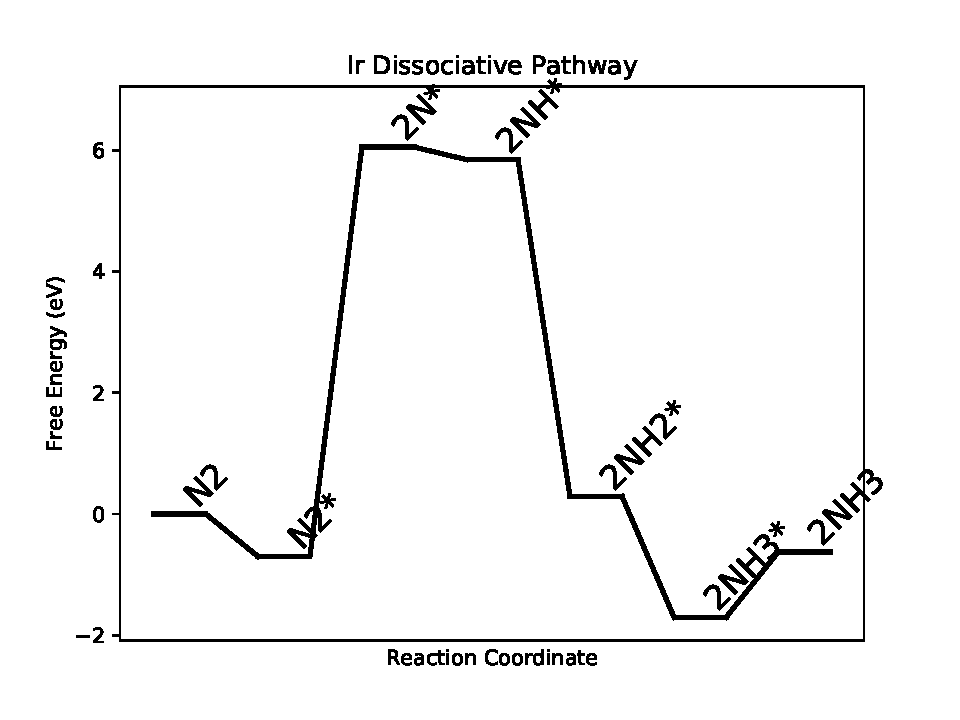
\includegraphics[width=0.5\linewidth]{data/plots/Ir_dissociative.pdf}
\label{fig:Ir_dissociative}
\end{figure}

\begin{figure}
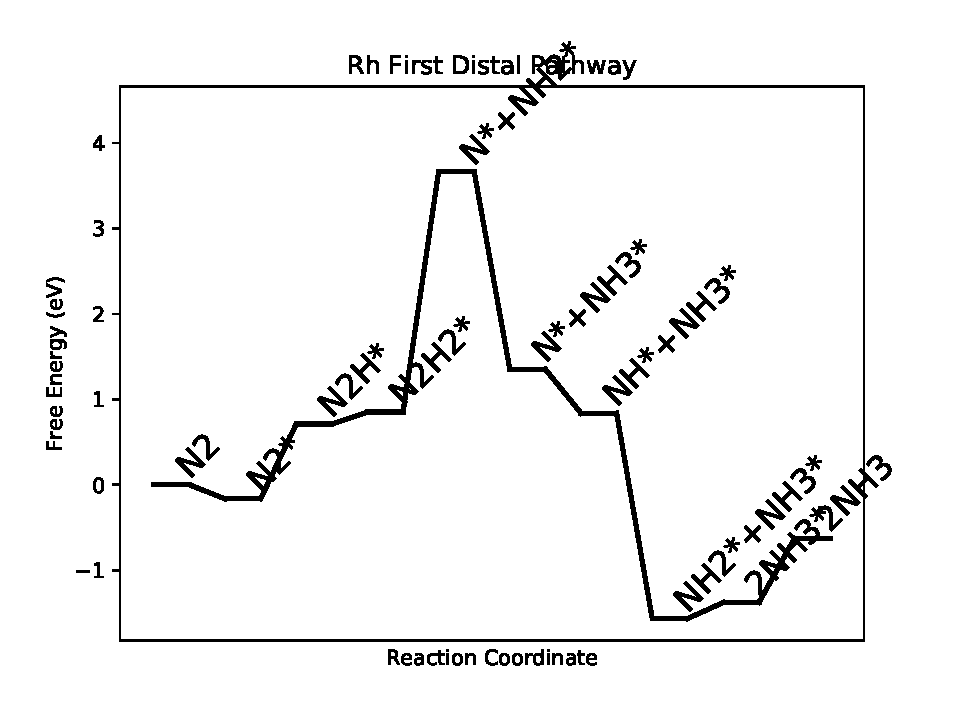
\includegraphics[width=0.5\linewidth]{data/plots/Rh_distal_1.pdf}
\label{fig:Rh_distal_1}
\end{figure}

\begin{figure}
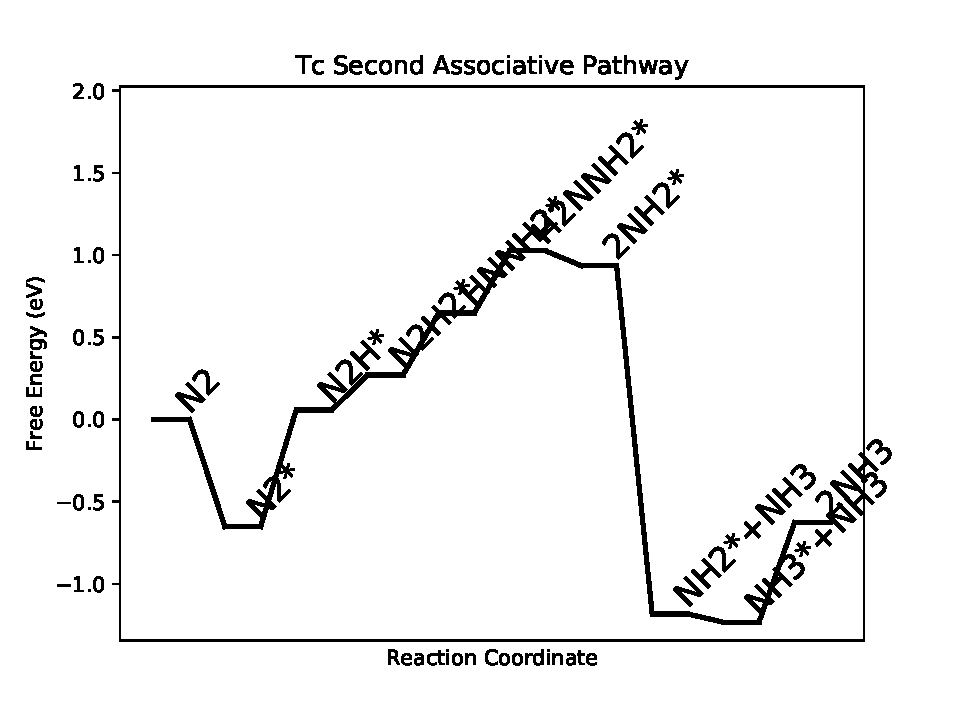
\includegraphics[width=0.5\linewidth]{data/plots/Tc_associative_2.pdf}
\label{fig:Tc_associative_2}
\end{figure}

\begin{figure}
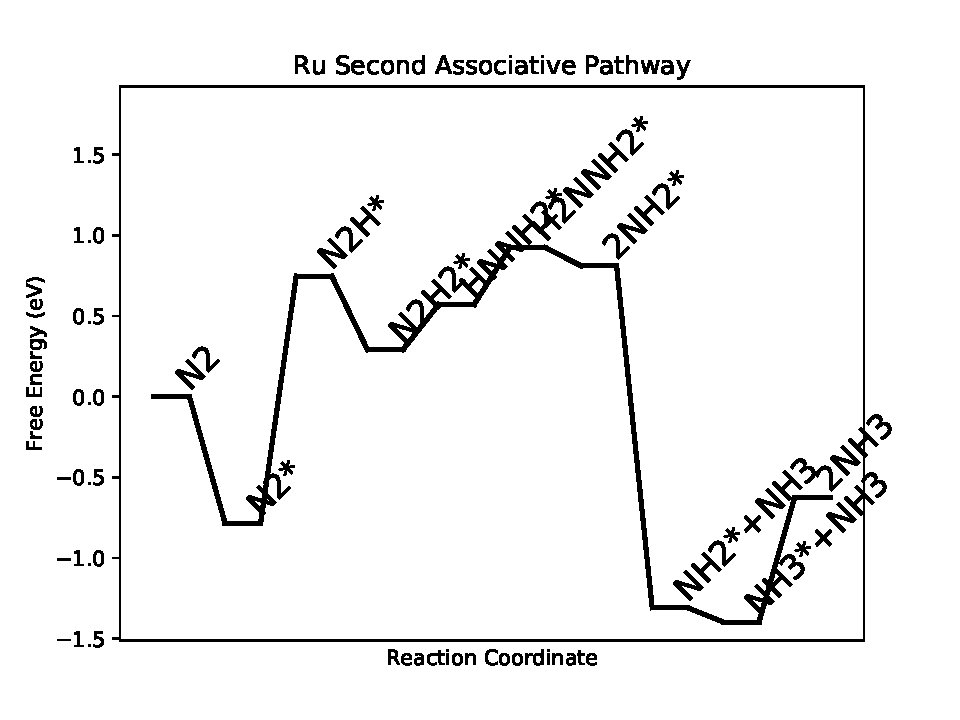
\includegraphics[width=0.5\linewidth]{data/plots/Ru_associative_2.pdf}
\label{fig:Ru_associative_2}
\end{figure}

\begin{figure}
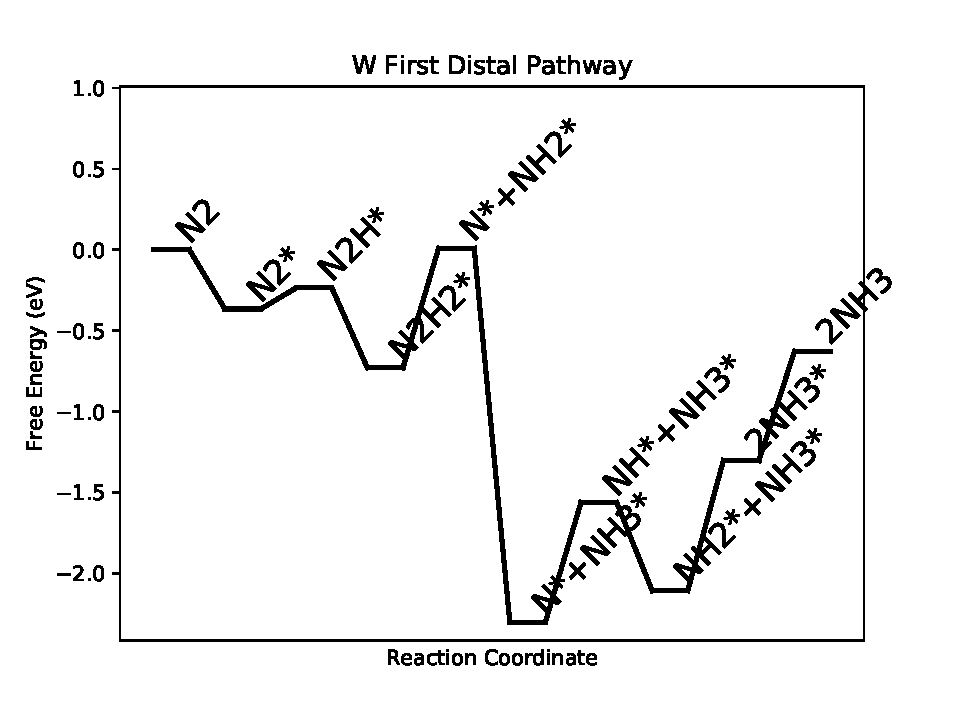
\includegraphics[width=0.5\linewidth]{data/plots/W_distal_1.pdf}
\label{fig:W_distal_1}
\end{figure}

\begin{figure}
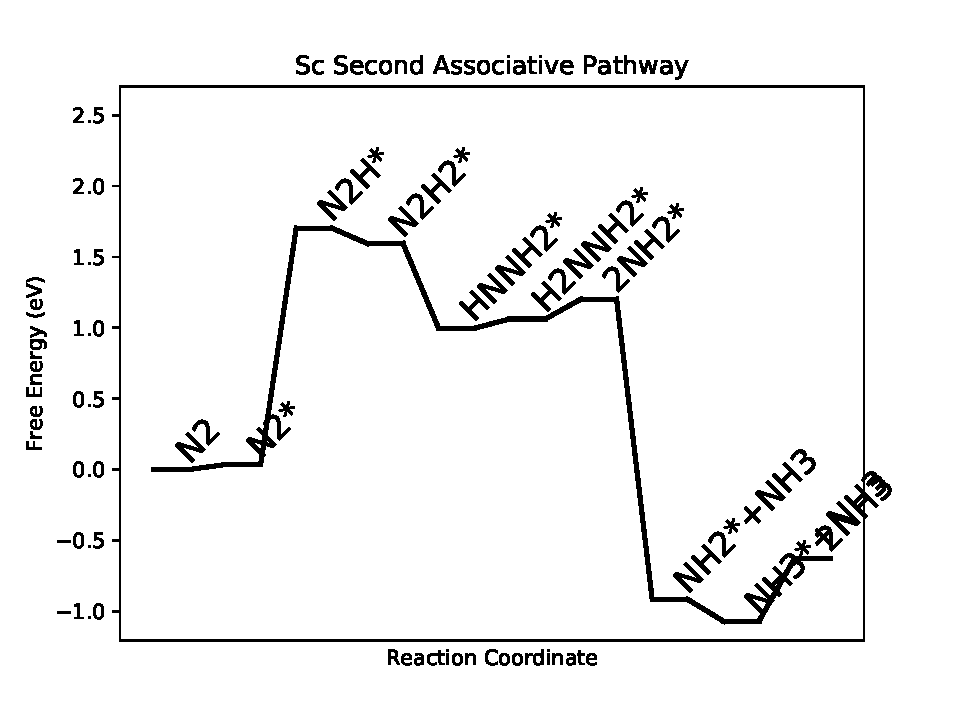
\includegraphics[width=0.5\linewidth]{data/plots/Sc_associative_2.pdf}
\label{fig:Sc_associative_2}
\end{figure}

\begin{figure}
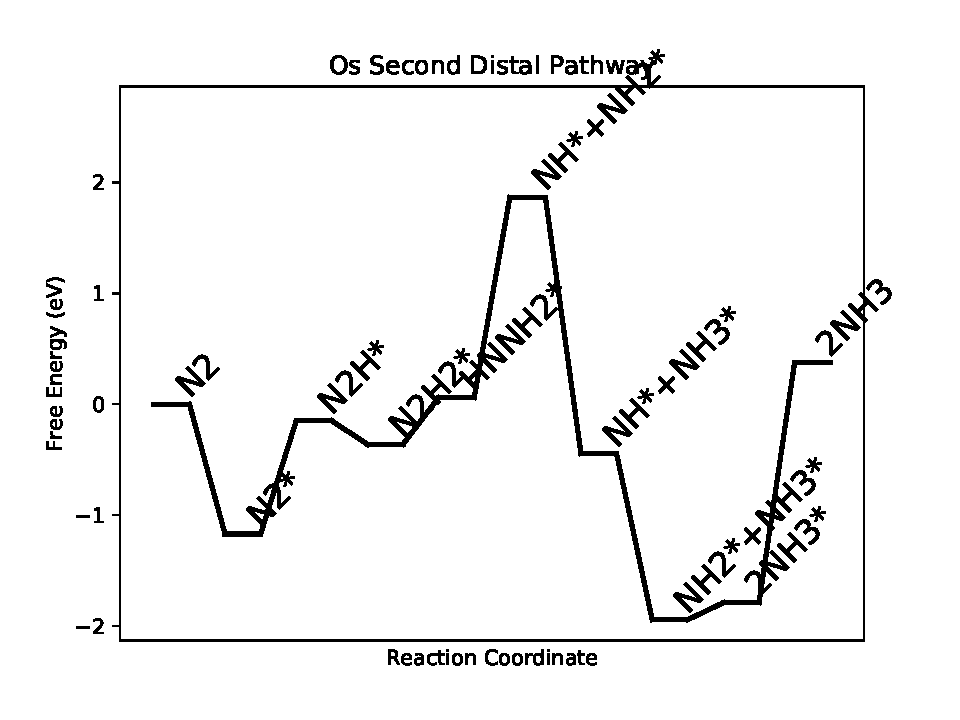
\includegraphics[width=0.5\linewidth]{data/plots/Os_distal_2.pdf}
\label{fig:Os_distal_2}
\end{figure}

\begin{figure}
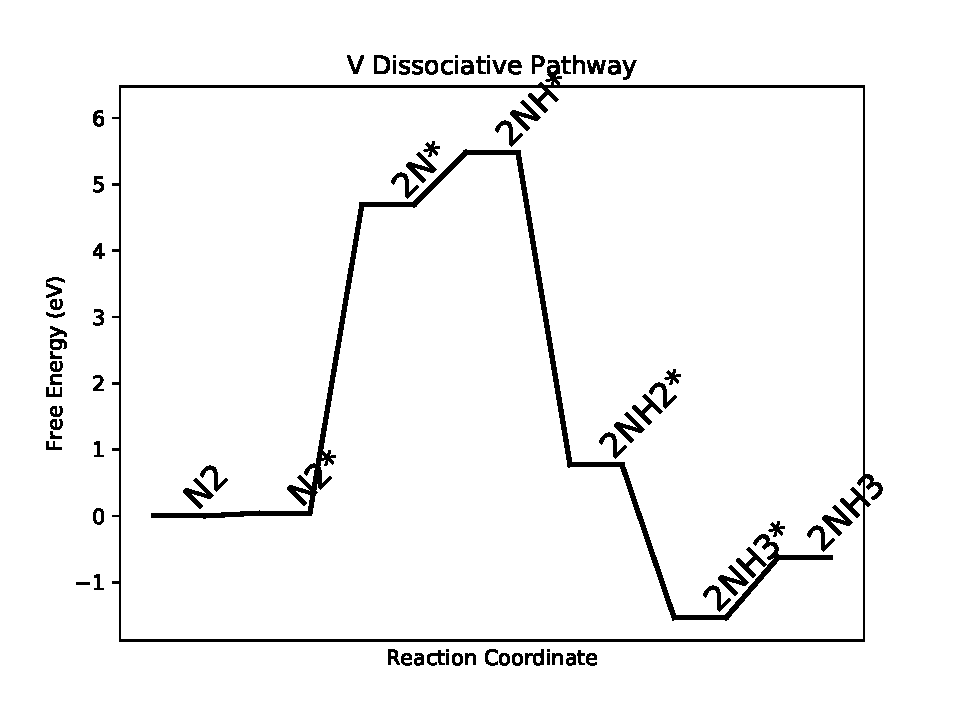
\includegraphics[width=0.5\linewidth]{data/plots/V_dissociative.pdf}
\label{fig:V_dissociative}
\end{figure}

\begin{figure}
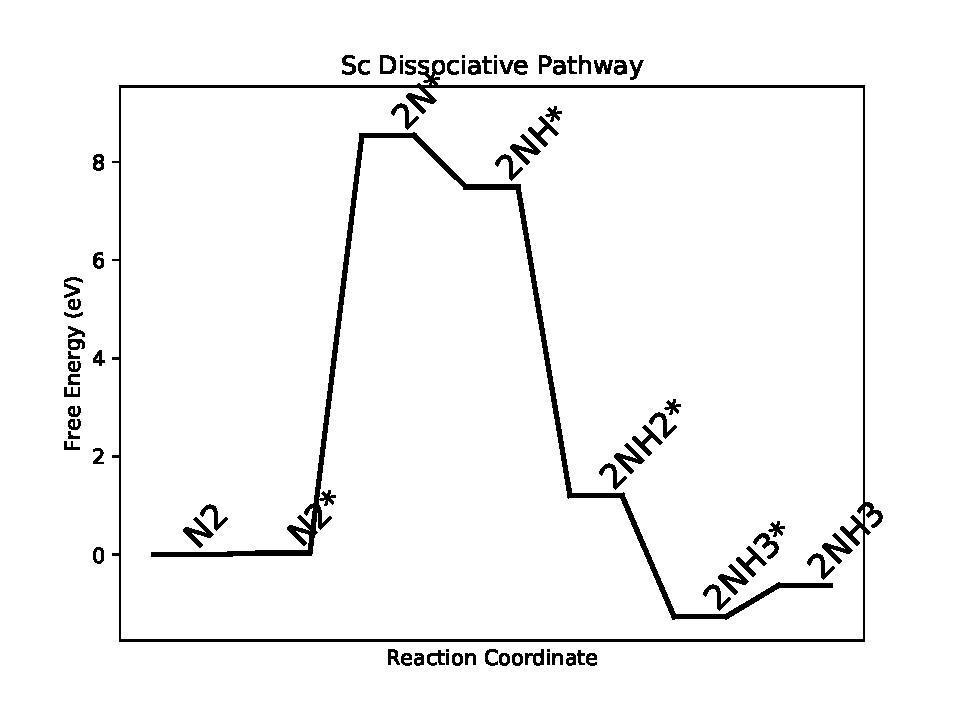
\includegraphics[width=0.5\linewidth]{data/plots/Sc_dissociative.pdf}
\label{fig:Sc_dissociative}
\end{figure}

\begin{figure}
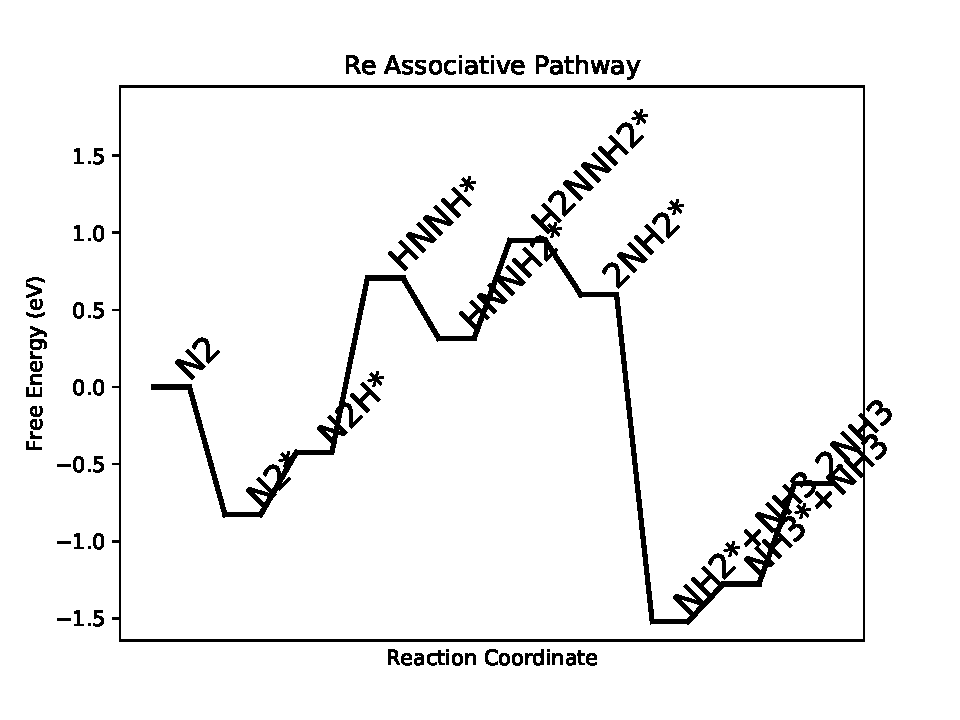
\includegraphics[width=0.5\linewidth]{data/plots/Re_associative.pdf}
\label{fig:Re_associative}
\end{figure}

\begin{figure}
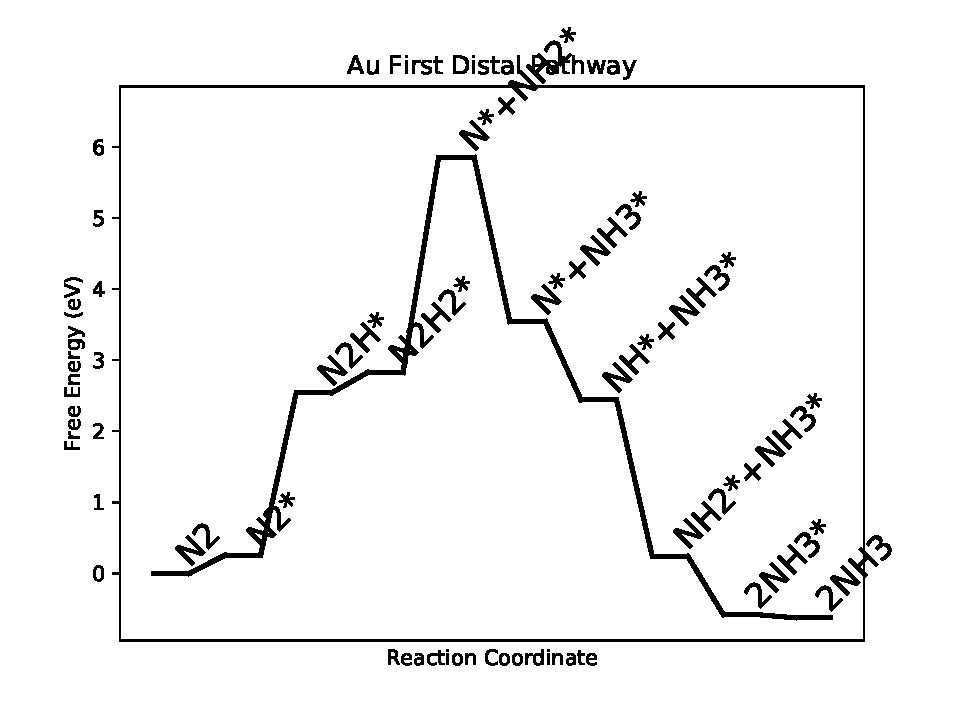
\includegraphics[width=0.5\linewidth]{data/plots/Au_distal_1.pdf}
\label{fig:Au_distal_1}
\end{figure}

\begin{figure}
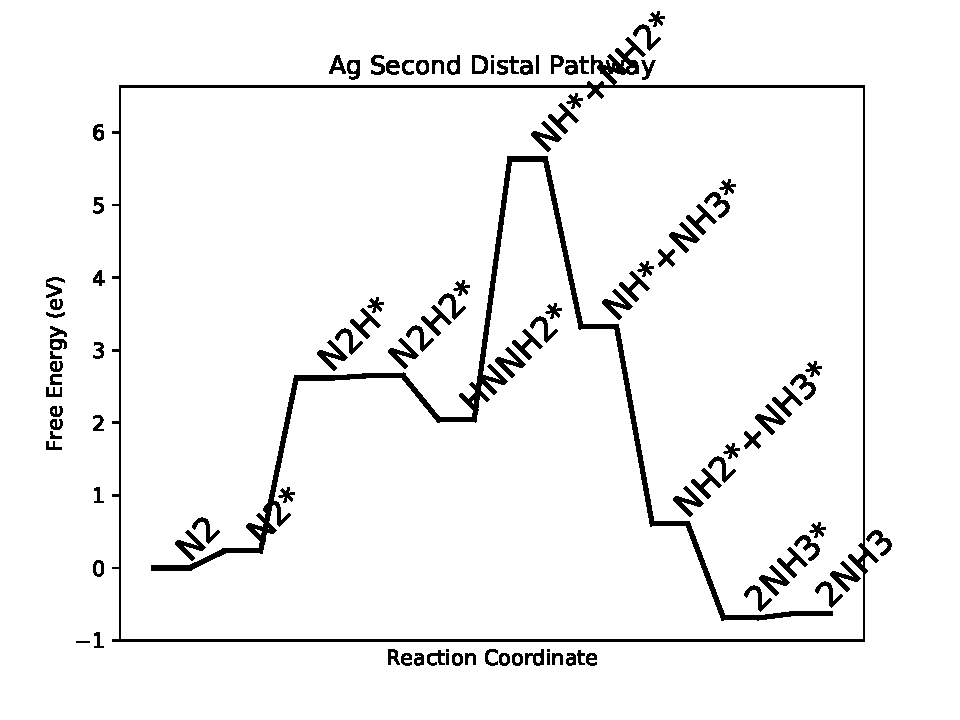
\includegraphics[width=0.5\linewidth]{data/plots/Ag_distal_2.pdf}
\label{fig:Ag_distal_2}
\end{figure}

\begin{figure}
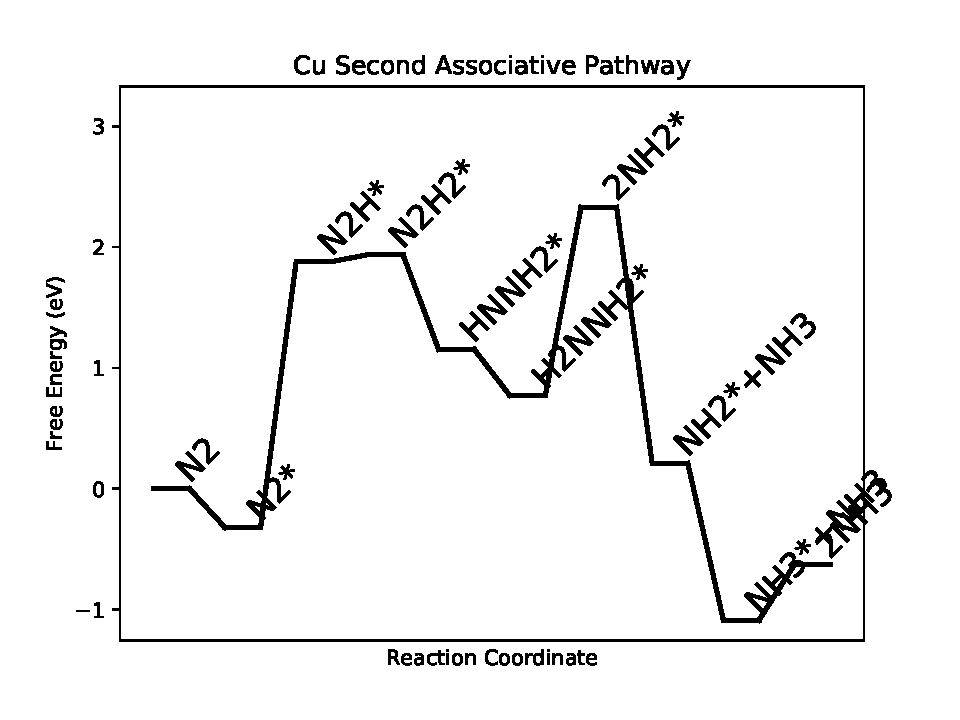
\includegraphics[width=0.5\linewidth]{data/plots/Cu_associative_2.pdf}
\label{fig:Cu_associative_2}
\end{figure}

\begin{figure}
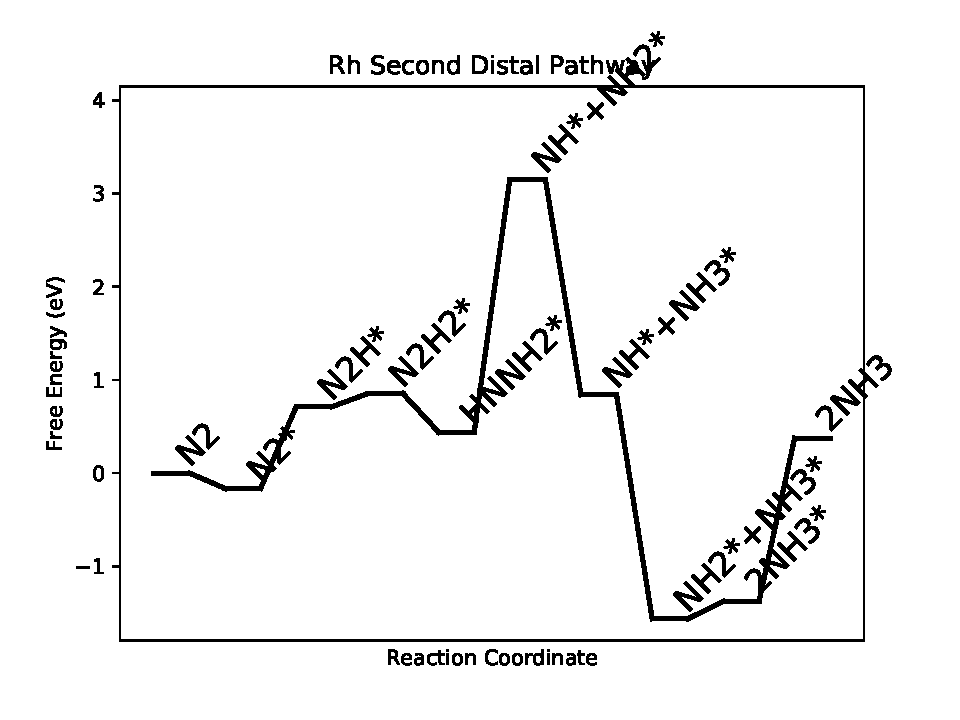
\includegraphics[width=0.5\linewidth]{data/plots/Rh_distal_2.pdf}
\label{fig:Rh_distal_2}
\end{figure}

\begin{figure}
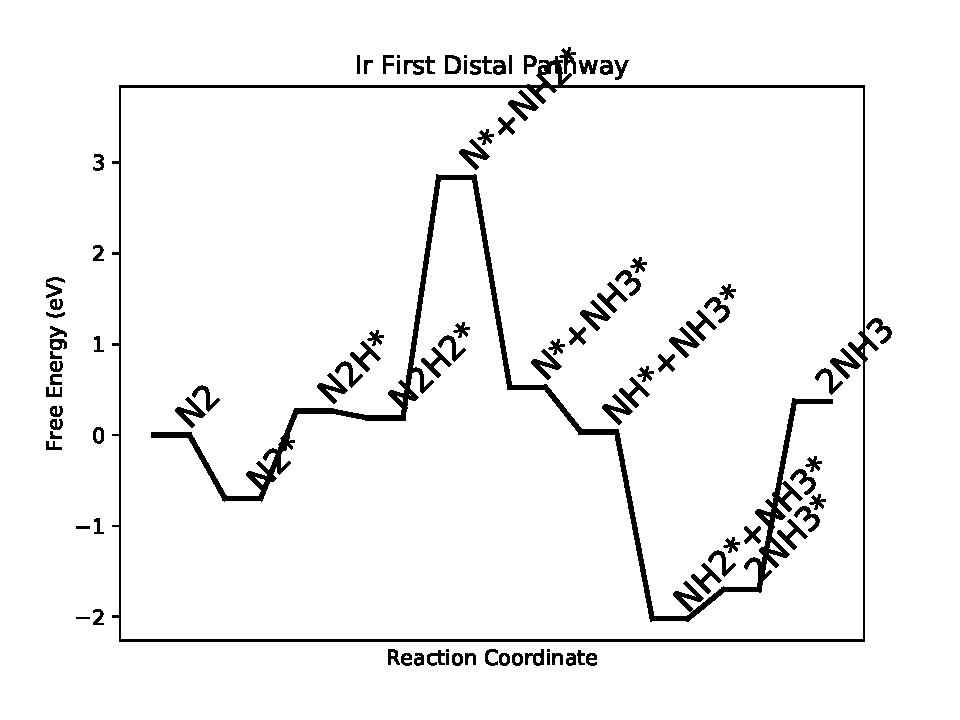
\includegraphics[width=0.5\linewidth]{data/plots/Ir_distal_1.pdf}
\label{fig:Ir_distal_1}
\end{figure}

\begin{figure}
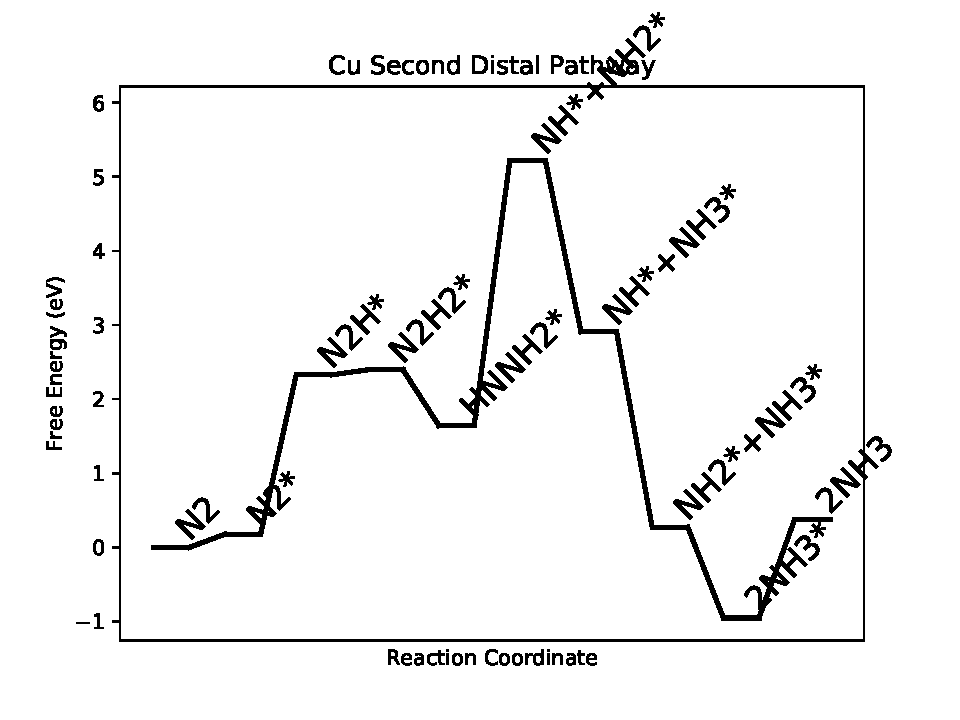
\includegraphics[width=0.5\linewidth]{data/plots/Cu_distal_2.pdf}
\label{fig:Cu_distal_2}
\end{figure}

\begin{figure}
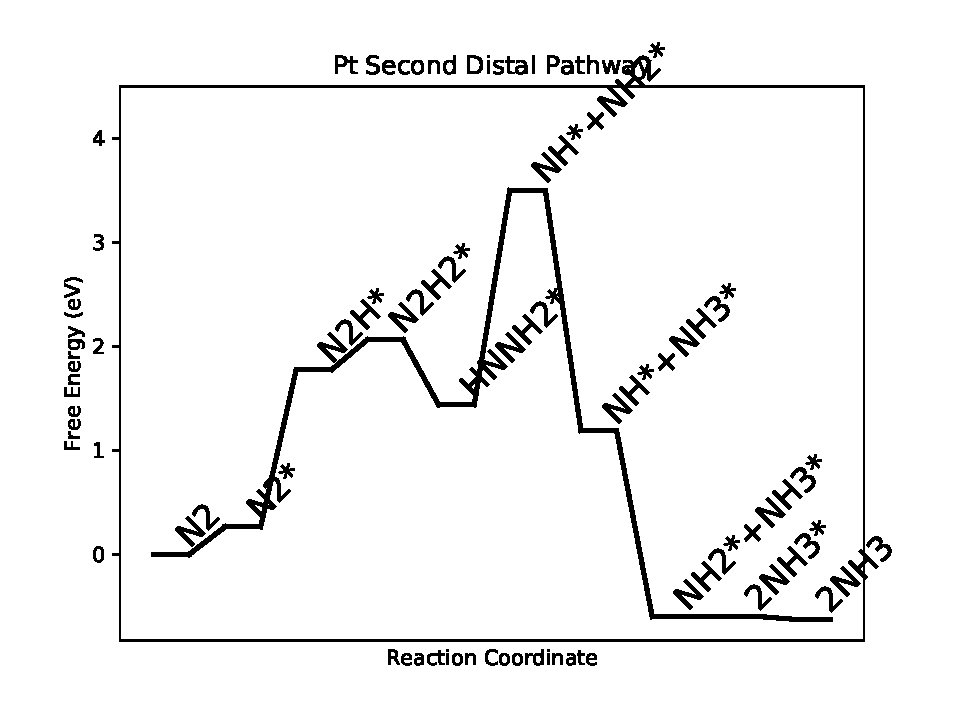
\includegraphics[width=0.5\linewidth]{data/plots/Pt_distal_2.pdf}
\label{fig:Pt_distal_2}
\end{figure}

\begin{figure}
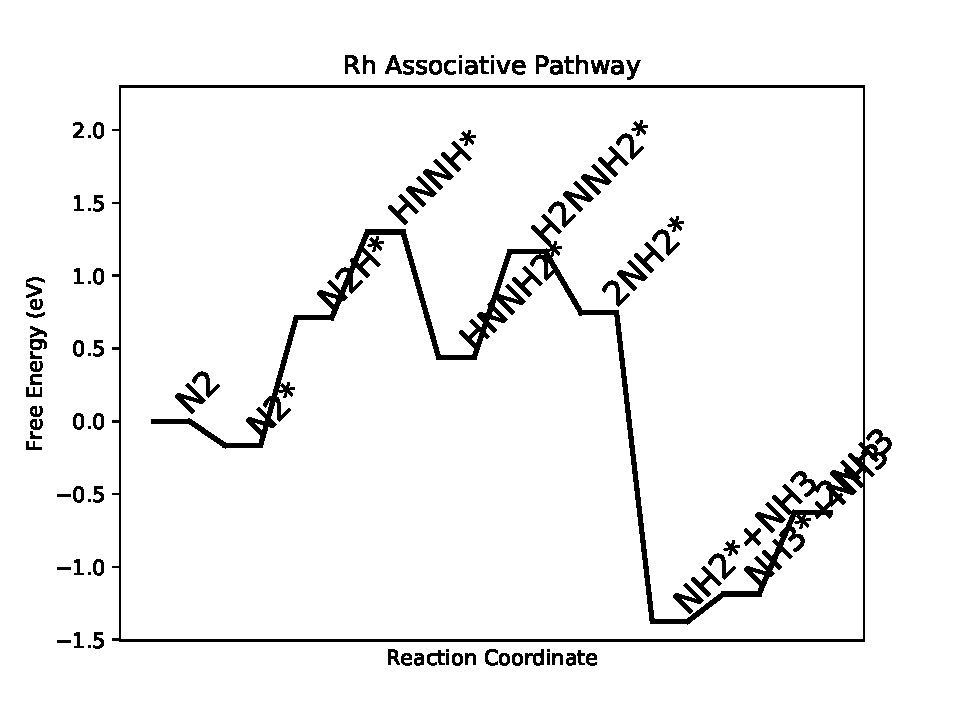
\includegraphics[width=0.5\linewidth]{data/plots/Rh_associative.pdf}
\label{fig:Rh_associative}
\end{figure}

\begin{figure}
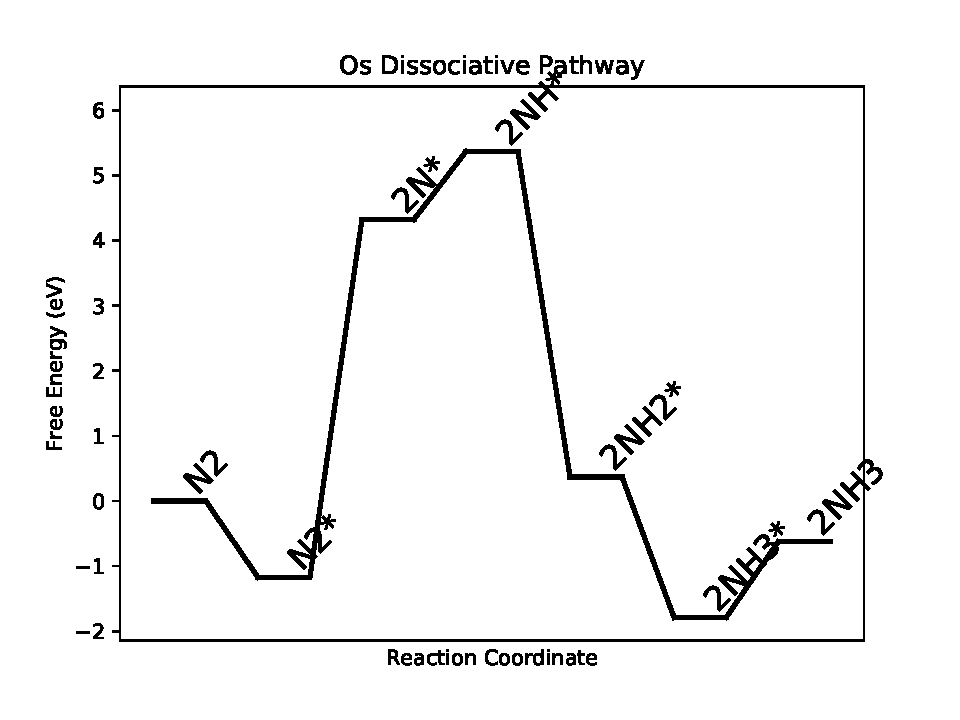
\includegraphics[width=0.5\linewidth]{data/plots/Os_dissociative.pdf}
\label{fig:Os_dissociative}
\end{figure}

\begin{figure}
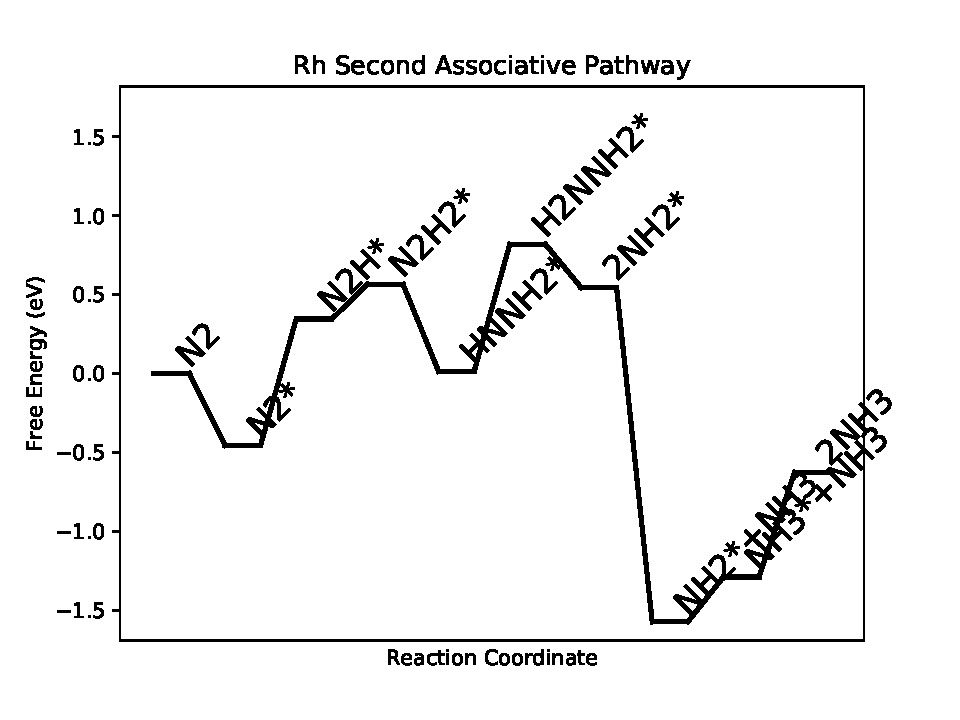
\includegraphics[width=0.5\linewidth]{data/plots/Rh_associative_2.pdf}
\label{fig:Rh_associative_2}
\end{figure}

\begin{figure}
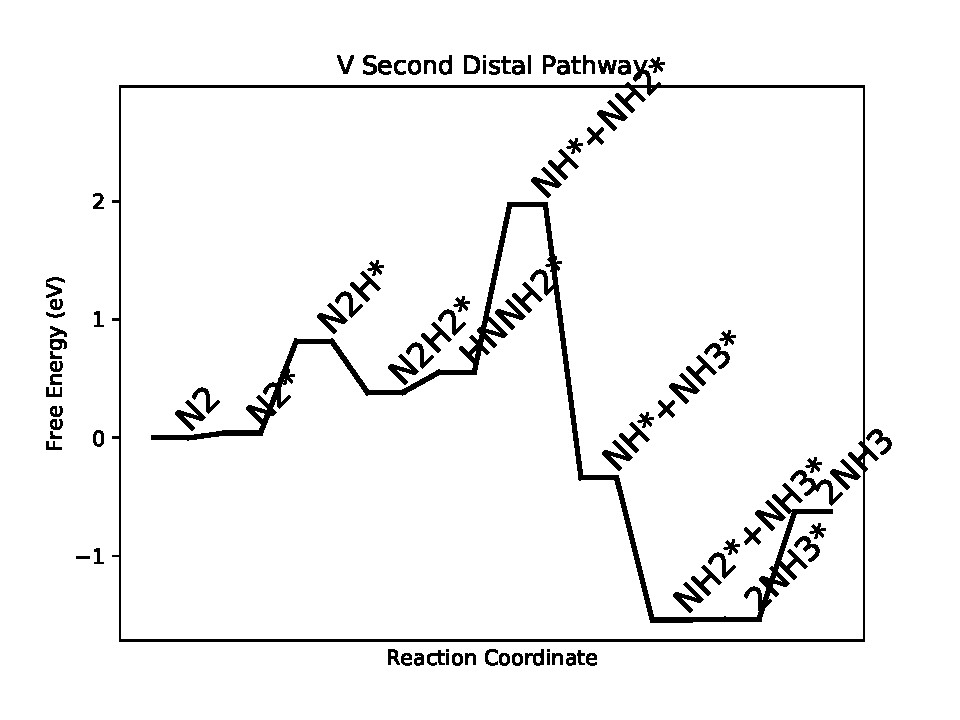
\includegraphics[width=0.5\linewidth]{data/plots/V_distal_2.pdf}
\label{fig:V_distal_2}
\end{figure}

\begin{figure}
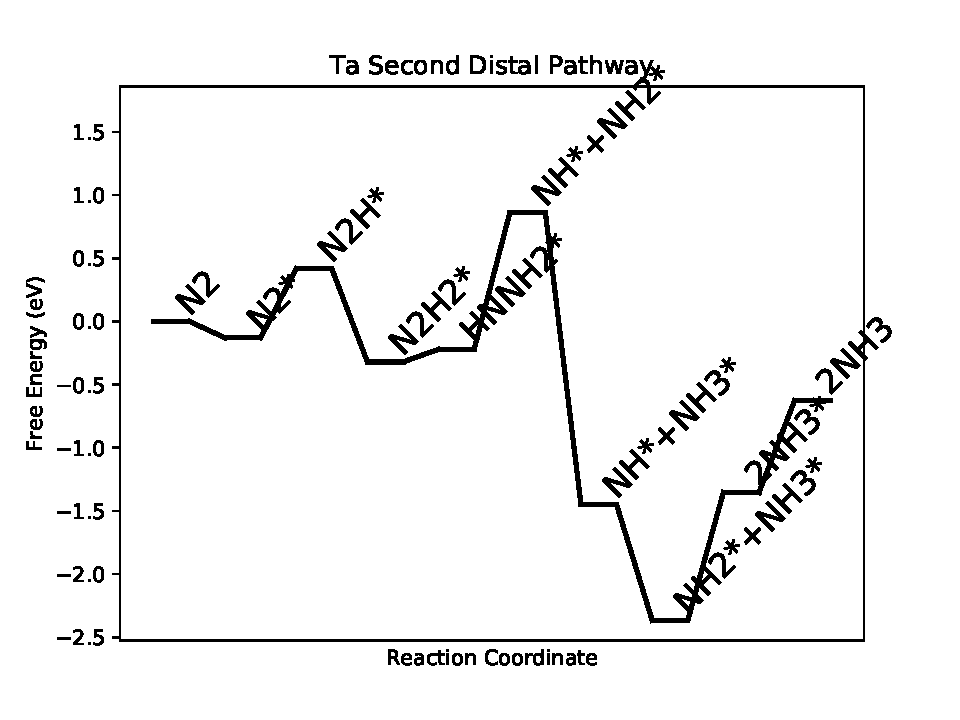
\includegraphics[width=0.5\linewidth]{data/plots/Ta_distal_2.pdf}
\label{fig:Ta_distal_2}
\end{figure}

\begin{figure}
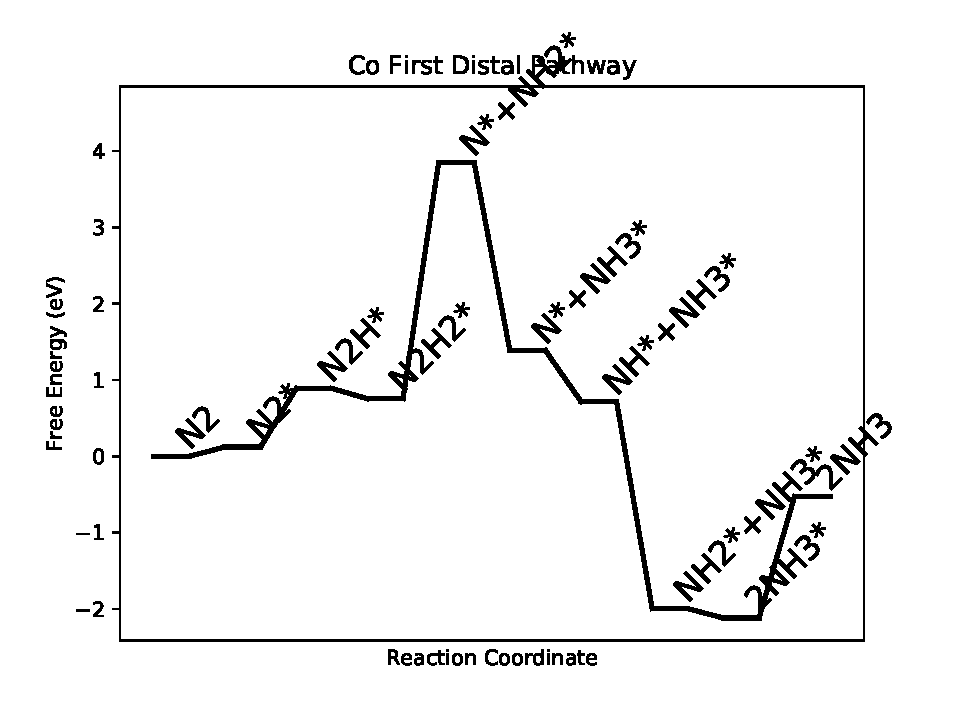
\includegraphics[width=0.5\linewidth]{data/plots/Co_distal_1.pdf}
\label{fig:Co_distal_1}
\end{figure}

\begin{figure}
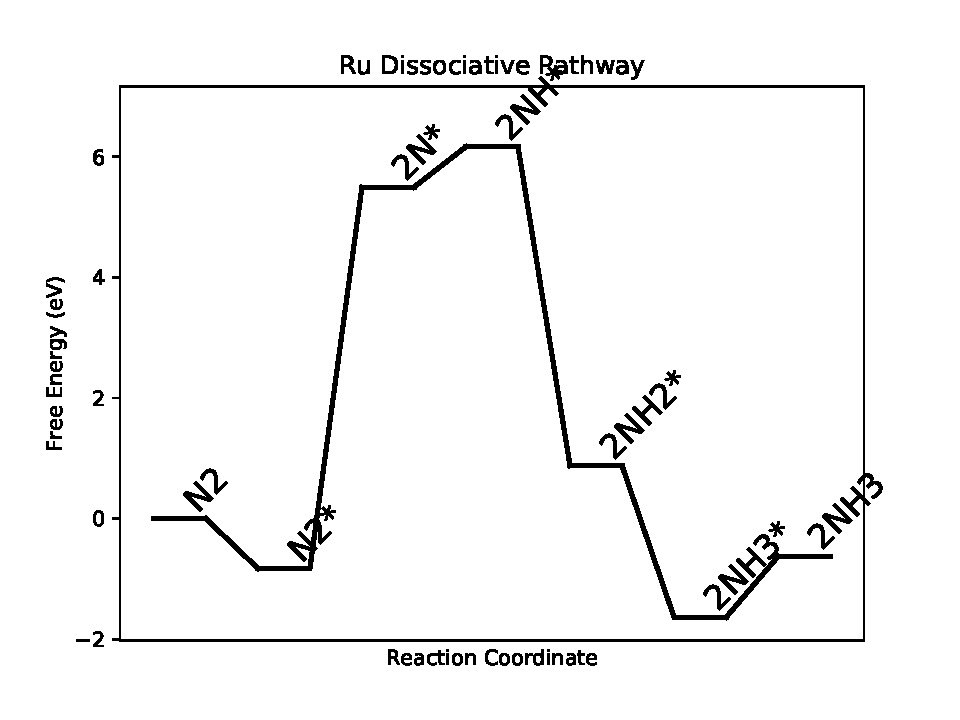
\includegraphics[width=0.5\linewidth]{data/plots/Ru_dissociative.pdf}
\label{fig:Ru_dissociative}
\end{figure}

\begin{figure}
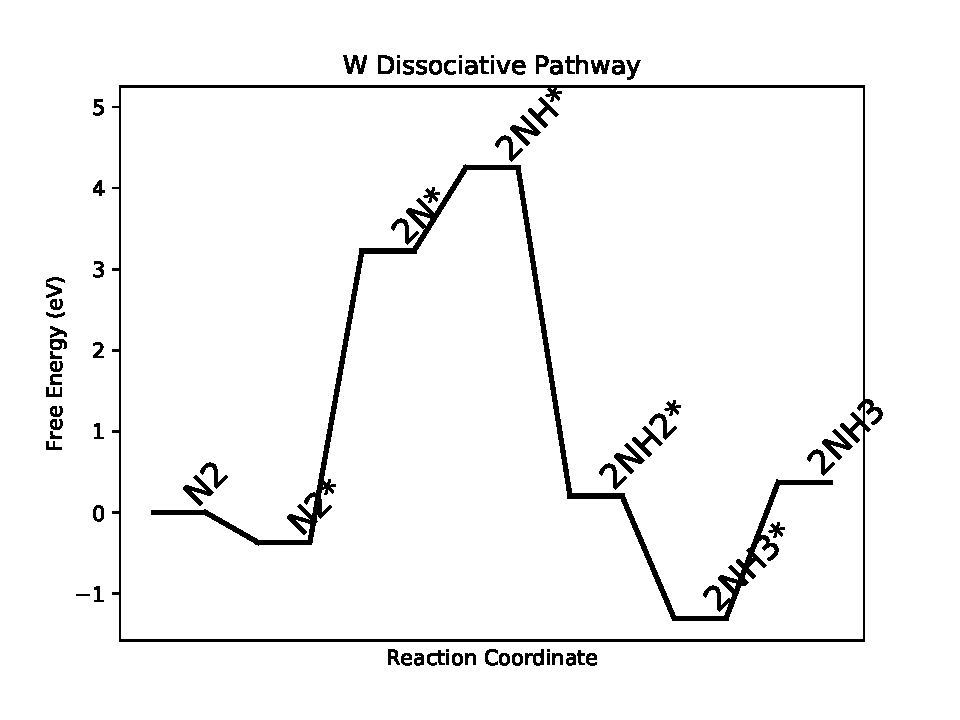
\includegraphics[width=0.5\linewidth]{data/plots/W_dissociative.pdf}
\label{fig:W_dissociative}
\end{figure}

\begin{figure}
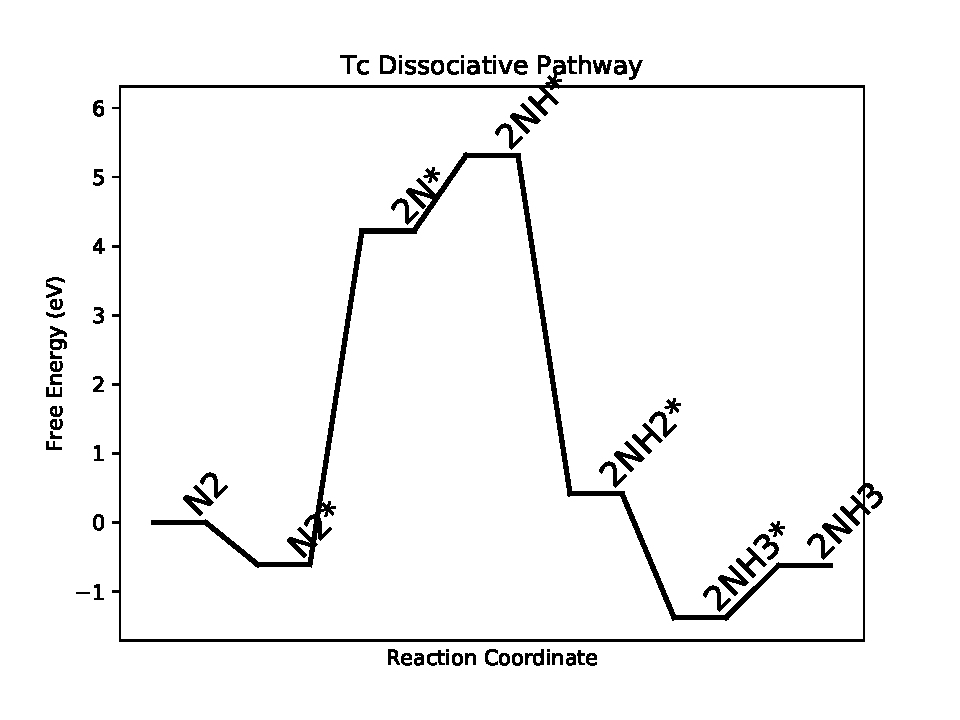
\includegraphics[width=0.5\linewidth]{data/plots/Tc_dissociative.pdf}
\label{fig:Tc_dissociative}
\end{figure}

\begin{figure}
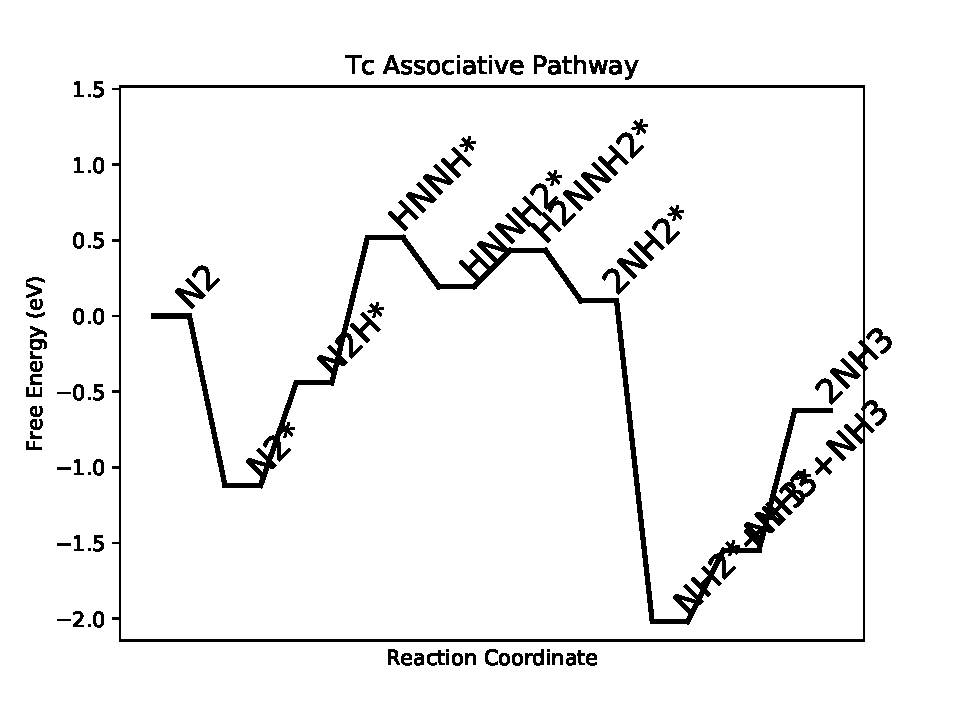
\includegraphics[width=0.5\linewidth]{data/plots/Tc_associative.pdf}
\label{fig:Tc_associative}
\end{figure}

\begin{figure}
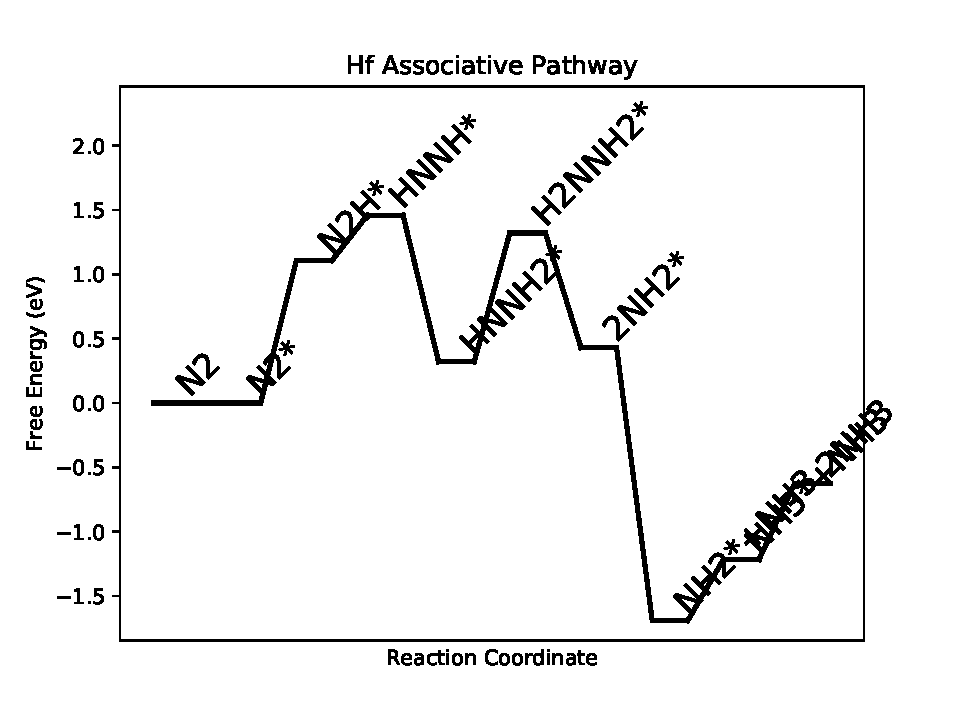
\includegraphics[width=0.5\linewidth]{data/plots/Hf_associative.pdf}
\label{fig:Hf_associative}
\end{figure}

\begin{figure}
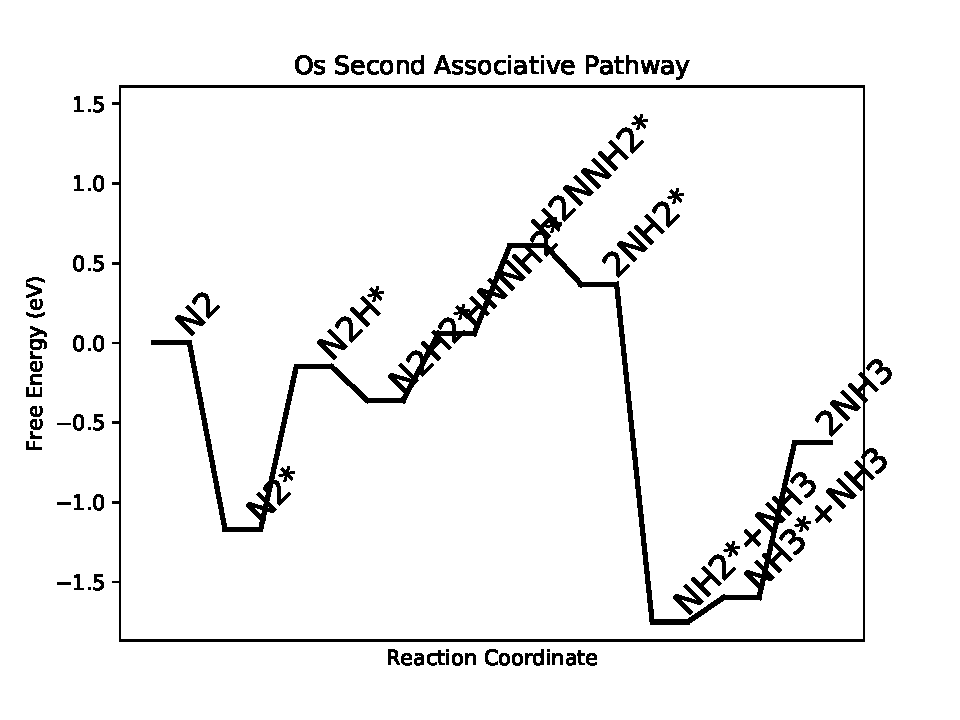
\includegraphics[width=0.5\linewidth]{data/plots/Os_associative_2.pdf}
\label{fig:Os_associative_2}
\end{figure}

\begin{figure}
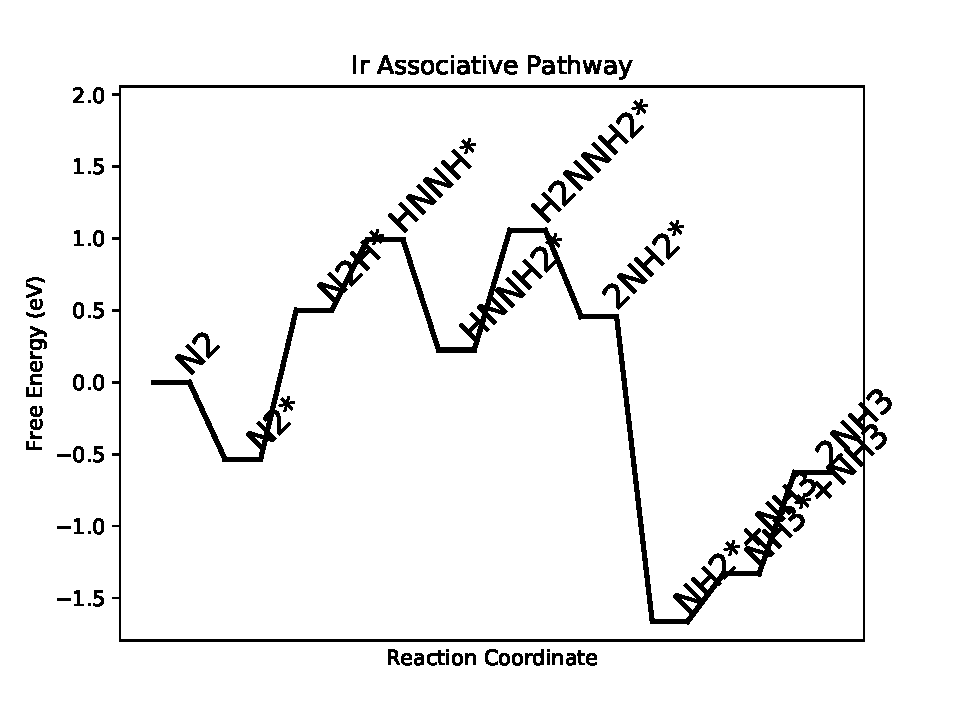
\includegraphics[width=0.5\linewidth]{data/plots/Ir_associative.pdf}
\label{fig:Ir_associative}
\end{figure}

\begin{figure}
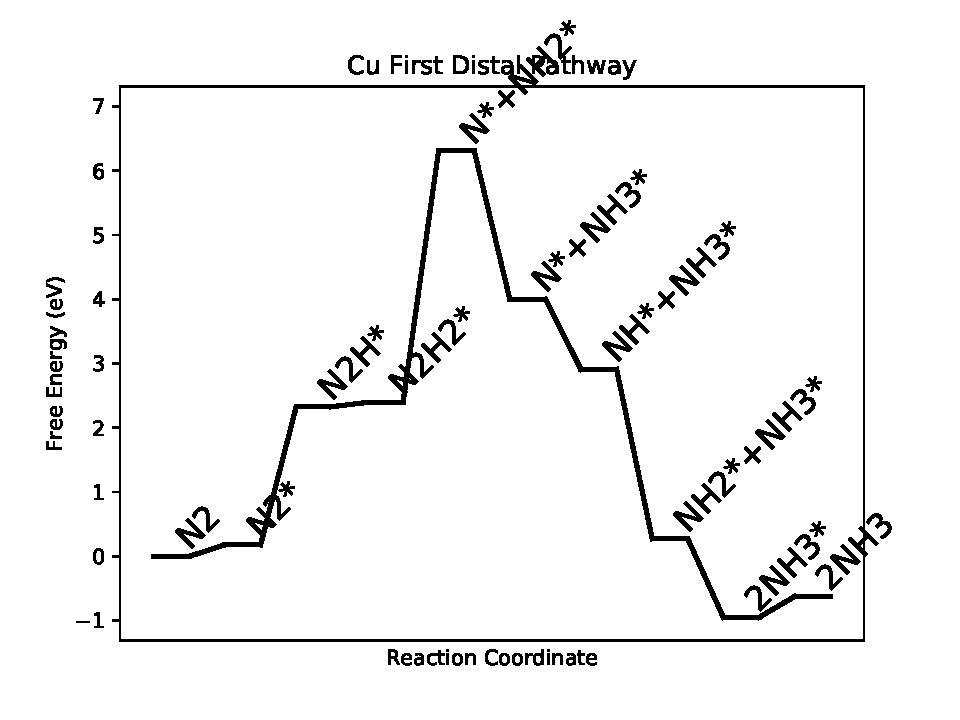
\includegraphics[width=0.5\linewidth]{data/plots/Cu_distal_1.pdf}
\label{fig:Cu_distal_1}
\end{figure}

\begin{figure}
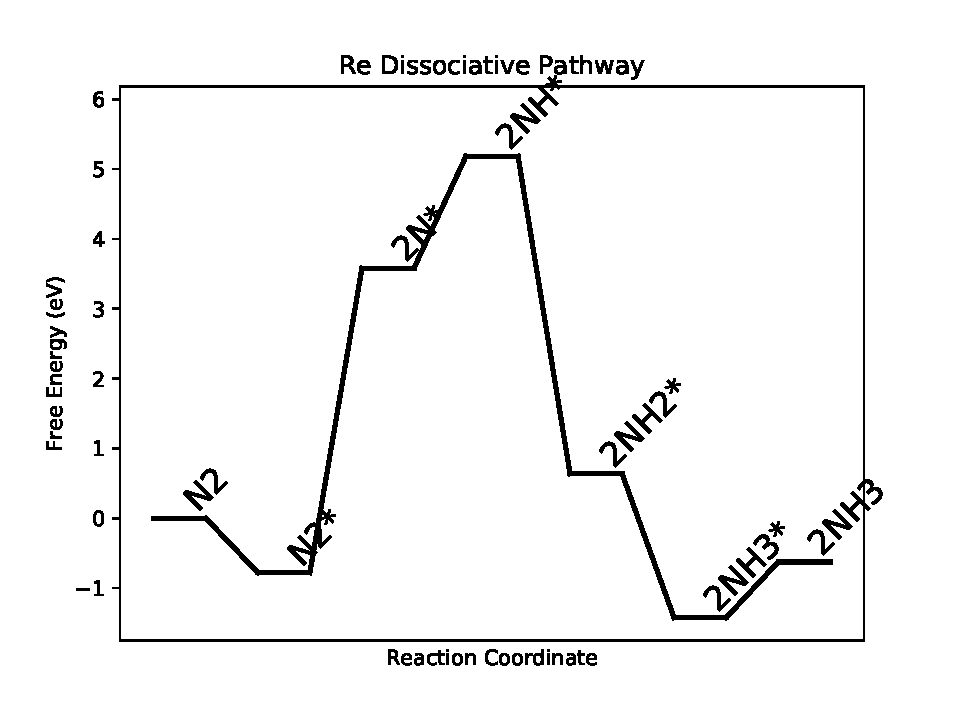
\includegraphics[width=0.5\linewidth]{data/plots/Re_dissociative.pdf}
\label{fig:Re_dissociative}
\end{figure}

\begin{figure}
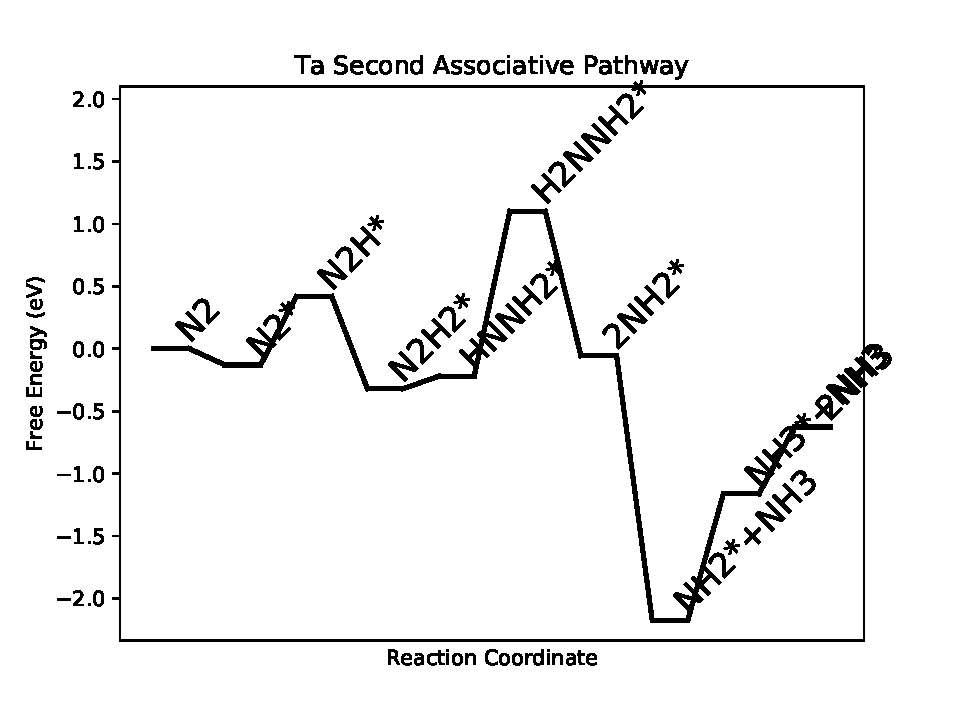
\includegraphics[width=0.5\linewidth]{data/plots/Ta_associative_2.pdf}
\label{fig:Ta_associative_2}
\end{figure}

\begin{figure}
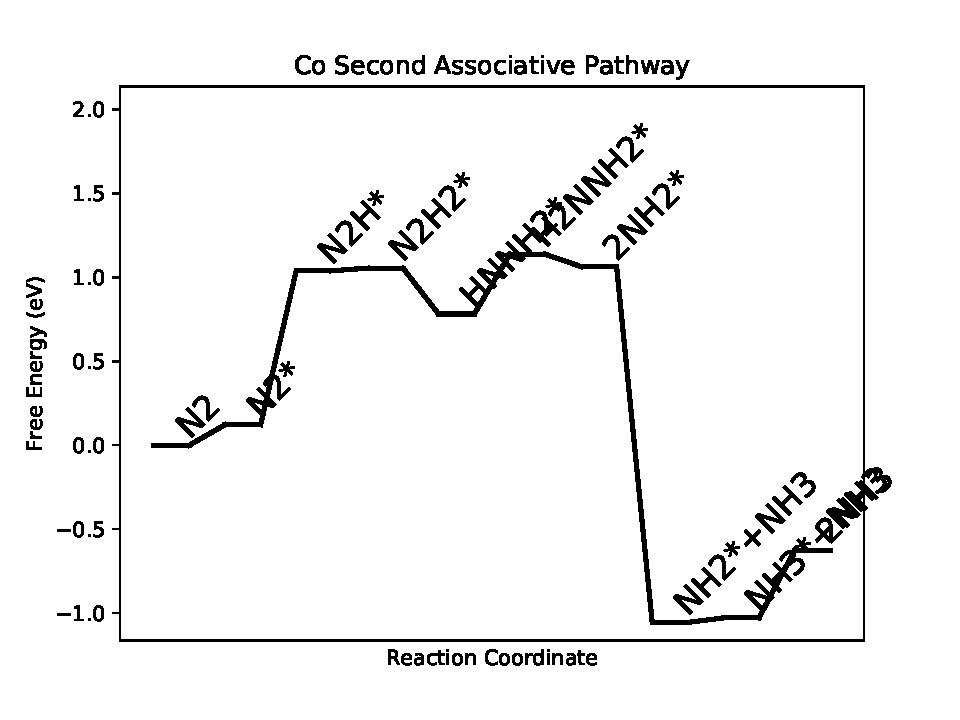
\includegraphics[width=0.5\linewidth]{data/plots/Co_associative_2.pdf}
\label{fig:Co_associative_2}
\end{figure}

\begin{figure}
\includegraphics[width=0.5\linewidth]{data/plots/Mo_associative_2.pdf}
\label{fig:Mo_associative_2}
\end{figure}

\begin{figure}
\includegraphics[width=0.5\linewidth]{data/plots/Nb_associative.pdf}
\label{fig:Nb_associative}
\end{figure}

\begin{figure}
\includegraphics[width=0.5\linewidth]{data/plots/Pd_associative.pdf}
\label{fig:Pd_associative}
\end{figure}

\begin{figure}
\includegraphics[width=0.5\linewidth]{data/plots/Tc_distal_2.pdf}
\label{fig:Tc_distal_2}
\end{figure}

\begin{figure}
\includegraphics[width=0.5\linewidth]{data/plots/Co_dissociative.pdf}
\label{fig:Co_dissociative}
\end{figure}

\begin{figure}
\includegraphics[width=0.5\linewidth]{data/plots/Mo_associative.pdf}
\label{fig:Mo_associative}
\end{figure}

\begin{figure}
\includegraphics[width=0.5\linewidth]{data/plots/Pd_distal_2.pdf}
\label{fig:Pd_distal_2}
\end{figure}

\begin{figure}
\includegraphics[width=0.5\linewidth]{data/plots/Nb_associative_2.pdf}
\label{fig:Nb_associative_2}
\end{figure}

\begin{figure}
\includegraphics[width=0.5\linewidth]{data/plots/W_associative.pdf}
\label{fig:W_associative}
\end{figure}

\begin{figure}
\includegraphics[width=0.5\linewidth]{data/plots/Ag_dissociative.pdf}
\label{fig:Ag_dissociative}
\end{figure}

\begin{figure}
\includegraphics[width=0.5\linewidth]{data/plots/Y_dissociative.pdf}
\label{fig:Y_dissociative}
\end{figure}

\begin{figure}
\includegraphics[width=0.5\linewidth]{data/plots/Nb_dissociative.pdf}
\label{fig:Nb_dissociative}
\end{figure}

\begin{figure}
\includegraphics[width=0.5\linewidth]{data/plots/Sc_distal_1.pdf}
\label{fig:Sc_distal_1}
\end{figure}

\begin{figure}
\includegraphics[width=0.5\linewidth]{data/plots/Nb_distal_2.pdf}
\label{fig:Nb_distal_2}
\end{figure}

\begin{figure}
\includegraphics[width=0.5\linewidth]{data/plots/W_distal_2.pdf}
\label{fig:W_distal_2}
\end{figure}

\begin{figure}
\includegraphics[width=0.5\linewidth]{data/plots/Ta_dissociative.pdf}
\label{fig:Ta_dissociative}
\end{figure}

\begin{figure}
\includegraphics[width=0.5\linewidth]{data/plots/Tc_distal_1.pdf}
\label{fig:Tc_distal_1}
\end{figure}

\begin{figure}
\includegraphics[width=0.5\linewidth]{data/plots/Re_distal_1.pdf}
\label{fig:Re_distal_1}
\end{figure}

\begin{figure}
\includegraphics[width=0.5\linewidth]{data/plots/Ti_associative_2.pdf}
\label{fig:Ti_associative_2}
\end{figure}

\begin{figure}
\includegraphics[width=0.5\linewidth]{data/plots/Ru_distal_1.pdf}
\label{fig:Ru_distal_1}
\end{figure}

\begin{figure}
\includegraphics[width=0.5\linewidth]{data/plots/V_associative.pdf}
\label{fig:V_associative}
\end{figure}

\begin{figure}
\includegraphics[width=0.5\linewidth]{data/plots/Ni_associative.pdf}
\label{fig:Ni_associative}
\end{figure}

\begin{figure}
\includegraphics[width=0.5\linewidth]{data/plots/Hf_associative_2.pdf}
\label{fig:Hf_associative_2}
\end{figure}

\begin{figure}
\includegraphics[width=0.5\linewidth]{data/plots/Re_associative_2.pdf}
\label{fig:Re_associative_2}
\end{figure}

\begin{figure}
\includegraphics[width=0.5\linewidth]{data/plots/Ir_associative_2.pdf}
\label{fig:Ir_associative_2}
\end{figure}

\begin{figure}
\includegraphics[width=0.5\linewidth]{data/plots/Ag_associative_2.pdf}
\label{fig:Ag_associative_2}
\end{figure}

\begin{figure}
\includegraphics[width=0.5\linewidth]{data/plots/Hf_distal_2.pdf}
\label{fig:Hf_distal_2}
\end{figure}

\begin{figure}
\includegraphics[width=0.5\linewidth]{data/plots/Re_distal_2.pdf}
\label{fig:Re_distal_2}
\end{figure}

\begin{figure}
\includegraphics[width=0.5\linewidth]{data/plots/Au_distal_2.pdf}
\label{fig:Au_distal_2}
\end{figure}

\begin{figure}
\includegraphics[width=0.5\linewidth]{data/plots/Sc_associative.pdf}
\label{fig:Sc_associative}
\end{figure}

\begin{figure}
\includegraphics[width=0.5\linewidth]{data/plots/Ti_distal_2.pdf}
\label{fig:Ti_distal_2}
\end{figure}

\begin{figure}
\includegraphics[width=0.5\linewidth]{data/plots/Mo_dissociative.pdf}
\label{fig:Mo_dissociative}
\end{figure}

\begin{figure}
\includegraphics[width=0.5\linewidth]{data/plots/Zr_dissociative.pdf}
\label{fig:Zr_dissociative}
\end{figure}

\begin{figure}
\includegraphics[width=0.5\linewidth]{data/plots/Ru_associative.pdf}
\label{fig:Ru_associative}
\end{figure}

\begin{figure}
\includegraphics[width=0.5\linewidth]{data/plots/Ag_distal_1.pdf}
\label{fig:Ag_distal_1}
\end{figure}

\begin{figure}
\includegraphics[width=0.5\linewidth]{data/plots/Os_associative.pdf}
\label{fig:Os_associative}
\end{figure}

\begin{figure}
\includegraphics[width=0.5\linewidth]{data/plots/Ag_associative.pdf}
\label{fig:Ag_associative}
\end{figure}

\begin{figure}
\includegraphics[width=0.5\linewidth]{data/plots/Co_distal_2.pdf}
\label{fig:Co_distal_2}
\end{figure}

\begin{figure}
\includegraphics[width=0.5\linewidth]{data/plots/Ta_distal_1.pdf}
\label{fig:Ta_distal_1}
\end{figure}

\begin{figure}
\includegraphics[width=0.5\linewidth]{data/plots/Zr_distal_2.pdf}
\label{fig:Zr_distal_2}
\end{figure}

\begin{figure}
\includegraphics[width=0.5\linewidth]{data/plots/Ta_associative.pdf}
\label{fig:Ta_associative}
\end{figure}

\begin{figure}
\includegraphics[width=0.5\linewidth]{data/plots/Pt_distal_1.pdf}
\label{fig:Pt_distal_1}
\end{figure}

\begin{figure}
\includegraphics[width=0.5\linewidth]{data/plots/Cu_associative.pdf}
\label{fig:Cu_associative}
\end{figure}

\begin{figure}
\includegraphics[width=0.5\linewidth]{data/plots/Pd_associative_2.pdf}
\label{fig:Pd_associative_2}
\end{figure}

\begin{figure}
\includegraphics[width=0.5\linewidth]{data/plots/Pd_dissociative.pdf}
\label{fig:Pd_dissociative}
\end{figure}

\begin{figure}
\includegraphics[width=0.5\linewidth]{data/plots/Co_associative.pdf}
\label{fig:Co_associative}
\end{figure}

\begin{figure}
\includegraphics[width=0.5\linewidth]{data/plots/Au_associative.pdf}
\label{fig:Au_associative}
\end{figure}

\begin{figure}
\includegraphics[width=0.5\linewidth]{data/plots/V_distal_1.pdf}
\label{fig:V_distal_1}
\end{figure}

\begin{figure}
\includegraphics[width=0.5\linewidth]{data/plots/Ti_dissociative.pdf}
\label{fig:Ti_dissociative}
\end{figure}

\begin{figure}
\includegraphics[width=0.5\linewidth]{data/plots/Mo_distal_2.pdf}
\label{fig:Mo_distal_2}
\end{figure}

\begin{figure}
\includegraphics[width=0.5\linewidth]{data/plots/Sc_distal_2.pdf}
\label{fig:Sc_distal_2}
\end{figure}

\begin{figure}
\includegraphics[width=0.5\linewidth]{data/plots/Zr_associative_2.pdf}
\label{fig:Zr_associative_2}
\end{figure}

\begin{figure}
\includegraphics[width=0.5\linewidth]{data/plots/Zr_associative.pdf}
\label{fig:Zr_associative}
\end{figure}

\begin{figure}
\includegraphics[width=0.5\linewidth]{data/plots/Os_distal_1.pdf}
\label{fig:Os_distal_1}
\end{figure}

\begin{figure}
\includegraphics[width=0.5\linewidth]{data/plots/Ti_distal_1.pdf}
\label{fig:Ti_distal_1}
\end{figure}

\begin{figure}
\includegraphics[width=0.5\linewidth]{data/plots/Hf_dissociative.pdf}
\label{fig:Hf_dissociative}
\end{figure}

\begin{figure}
\includegraphics[width=0.5\linewidth]{data/plots/W_associative_2.pdf}
\label{fig:W_associative_2}
\end{figure}

\begin{figure}
\includegraphics[width=0.5\linewidth]{data/plots/Zr_distal_1.pdf}
\label{fig:Zr_distal_1}
\end{figure}

\begin{figure}
\includegraphics[width=0.5\linewidth]{data/plots/Hf_distal_1.pdf}
\label{fig:Hf_distal_1}
\end{figure}

\end{document}